%Este trabalho está licenciado sob a Licença Creative Commons Atribuição-CompartilhaIgual 3.0 Não Adaptada. Para ver uma cópia desta licença, visite http://creativecommons.org/licenses/by-sa/3.0/ ou envie uma carta para Creative Commons, PO Box 1866, Mountain View, CA 94042, USA.

%\documentclass[main.tex]{subfiles}
%\begin{document}

\chapter{Solução de equações de uma variável}\index{equações!de uma variável}

Neste capítulo, buscaremos aproximações numéricas para a solução de \emph{equações de uma variável real}. Observamos que obter uma solução para uma tal dada equação é equivalente a encontrar um \emph{zero de uma função}\index{função!zero de}\index{função!raiz de} apropriada. Com isso, iniciamos este capítulo discutindo sobre condições de existência e unicidade de raízes de funções de uma variável real. Então, apresentamos o \emph{método da bisseção}\index{método da bisseção} como uma primeira abordagem numérica para a solução de tais equações.

Em seguida, exploramos uma outra abordagem via \emph{iteração do ponto fixo}\index{iteração do ponto fixo}. Desta, obtemos o \emph{método de Newton}\footnote{Sir Isaac Newton, 1642 - 1727, matemático e físico inglês.}\index{método de Newton}, para o qual discutimos sua aplicação e convergência. Por fim, apresentamos o \emph{método das secantes}\index{método das secantes} como uma das possíveis variações do método de Newton.

%%%%%%%%%%%%%%%%%%%%
% python
%%%%%%%%%%%%%%%%%%%%
\ifispython
Ao longo do capítulo, apresentamos algumas computações com \verb+Python+. Nestas, estaremos assumindo o que os seguintes módulos estão carregados:
\begin{verbatim}
>>> from __future__ import division
>>> import numpy as np
>>> import matplotlib.pyplot as plt
\end{verbatim}
A segunda instrução carrega a biblioteca de computação científica \href{http://www.numpy.org/}{numpy} e a terceira carrega a biblioteca gráfica \href{http://matplotlib.org/}{matplotlib}.
\fi

\section{Existência e unicidade}\index{função!}\index{função!zero}

O \emph{teorema de Bolzano}\footnote{Bernhard Placidus Johann Gonzal Nepomuk Bolzano, 1781 - 1848, matemático do Reino da Boêmia.}\index{teorema de!Bolzano} nos fornece condições suficientes para a existência do zero de uma função. Este é uma aplicação direta do \emph{teorema do valor intermediário}\index{teorema do valor intermediário}.

\begin{teo}[Teorema de Bolzano]\label{teo:teorema_de_Bolzano}
  Se $f:[a, b]\to\mathbb{R}$, $y = f(x)$, é uma função contínua tal que $f(a)\cdot f(b) < 0$, então existe $x^*\in (a, b)$ tal que $f(x^*) = 0$.
\end{teo}
\begin{proof}
  O resultado é uma consequência imediata do teorema do valor intermediário que estabelece que dada uma função contínua $f:[a, b]\to\mathbb{R}$, $y = f(x)$, tal que $f(a) < f(b)$ (ou $f(b) < f(a)$), então para qualquer $d\in \left(f(a), f(b)\right)$ (ou $k\in \left(f(b), f(a)\right)$) existe $x^*\in (a, b)$ tal que $f(x^*) = k$. Ou seja, nestas notações, se $f(a)\cdot f(b) < 0$, então $f(a) < 0 < f(b)$ (ou $f(b) < 0 < f(a)$). Logo, tomando $k = 0$, temos que existe $x^*\in (a, b)$ tal que $f(x^*) = k = 0$.
\end{proof}

Em outras palavras, se $f(x)$ é uma função contínua em um dado intervalo no qual ela troca de sinal, então ela têm pelo menos um zero neste intervalo (veja a Figura~\ref{fig:teorema_de_Bolzano}).

\begin{figure}
  \centering
  \includegraphics{./cap_equacao1d/pics/teorema_de_Bolzano/teorema_de_Bolzano.eps}
  \caption{Teorema de Bolzano.}
  \label{fig:teorema_de_Bolzano}
\end{figure}

% \begin{teo}[Teorema do Valor Intermediário]
% Se $f:[a,b]\to\mathbb{R}$ é um função contínua e $K$ for um número entre $f(a)$ e $f(b)$, então existe $c\in(a,b)$ para o qual $f(c)=K$.
% \end{teo}

% \begin{figure}[h!]
%   \centering
%   \includegraphics[scale=0.5]{./cap_equacao1d/pics/teorema_do_valor_intermediario/teorema_do_valor_intermediario.eps}
%   \caption{Teorema do valor intermediário}
%   \label{fig:teorema_do_valor_intermediario}
% \end{figure}

% Em particular, se $f(a)>0$ e $f(b)<0$, então $0\in [f(b),f(a)]$ e podemos garantir a existência de $c\in(a,b)$ tal que $f(c)=0$, i.e. existe uma raiz no intervalo $(a,b)$. A mesma afirmação é válida se $f(a)<0$ e $f(b)>0$. Em outras palavras, o Teorema do Valor Intermediário afirma que uma função contínua não pode mudar de sinal sem passar por zero.

\begin{ex}\label{ex:teorema_de_Bolzano}
Mostre que existe pelo menos uma solução da equação $e^x=x+2$ no intervalo $(-2,0)$.
\end{ex}
\begin{sol}
Primeiramente, observamos que resolver a equação $e^x = x+2$ é equivalente a resolver $f(x) = 0$ com $f(x)=e^x-x-2$. Agora, como $f(-2)=e^{-2}>0$ e $f(0)=-2<0$, temos do teorema de Bolzano que existe pelo menos um zero de $f(x)$ no intervalo $(-2, 0)$. E, portanto, existe pelo menos uma solução da equação dada no intervalo $(-2, 0)$.

%%%%%%%%%%%%%%%%%%%%
% scilab
%%%%%%%%%%%%%%%%%%%%
\ifisscilab
Podemos usar o \verb+Scilab+ para estudarmos esta função. Por exemplo, podemos definir a função $f(x)$ e computá-la nos extremos do intervalo dado com os seguintes comandos:
\begin{verbatim}
-->deff('y=f(x)','y=exp(x)-x-2')
-->f(-2),f(0)
 ans  =
    0.1353353  
 ans  =
  - 1.  
\end{verbatim}
Alternativamente (e com maior precisão), podemos verificar diretamente o sinal da função nos pontos desejados com comando \verb+sign+:
\begin{verbatim}
-->sign(f(-2)),sign(f(0))
 ans  =
    1.  
 ans  =
  - 1.  
\end{verbatim}
\fi
%%%%%%%%%%%%%%%%%%%%
%%%%%%%%%%%%%%%%%%%%
% python
%%%%%%%%%%%%%%%%%%%%
\ifispython
Podemos usar \verb+Python+ para estudarmos esta função. Por exemplo, podemos definir a função $f(x)$ e computá-la nos extremos do intervalo dado com os seguintes comandos:
\begin{verbatim}
>>> def f(x): return np.exp(x)-x-2
... 
>>> f(-2),f(0)
(0.13533528323661281, -1.0)
\end{verbatim}
Alternativamente (e com maior precisão), podemos verificar diretamente o sinal da função nos pontos desejados com a função \href{https://docs.scipy.org/doc/numpy/reference/generated/numpy.sign.html?highlight=numpy.sign#numpy.sign}{numpy.sign}:
\begin{verbatim}
>>> np.sign(f(-2)*f(0))
-1.0
\end{verbatim}
\fi
%%%%%%%%%%%%%%%%%%%%
\end{sol}


Quando procuramos aproximações para zeros de funções, é aconselhável isolar cada raiz em um intervalo. Desta forma, gostaríamos de poder garantir a existência e a unicidade da raiz dentro de um dado intervalo. A seguinte proposição nos fornece condições suficientes para tanto.

\begin{prop}\label{prop:existencia_e_unicidade}
Se $f:[a, b]\to\mathbb{R}$ é um função diferenciável, $f(a)\cdot f(b)<0$ e $f'(x)>0$ (ou $f'(x)<0$) para todo $x\in(a, b)$, então existe um único $x^*\in (a, b)$ tal que $f(x^*) = 0$.
\end{prop}

Em outras palavras, para garantirmos que exista um único zero de uma dada função diferenciável num intervalo, é suficiente que ela troque de sinal e seja monótona neste intervalo.

\begin{ex}
No Exemplo~\ref{ex:teorema_de_Bolzano}, mostramos que existe pelo menos um zero de $f(x) = e^{x}-x-2$ no intervalo $(-2,0)$, pois $f(x)$ é contínua e $f(-2)\cdot f(0) < 0$. Agora, observamos que, além disso, $f'(x)=e^x-1$ e, portanto, $f'(x)<0$ para todo $x\in(-2,0)$. Logo, da Proposição~\ref{prop:existencia_e_unicidade}, temos garantida a existência de um único zero no intervalo dado.

%%%%%%%%%%%%%%%%%%%%
% scilab
%%%%%%%%%%%%%%%%%%%%
\ifisscilab
Podemos inspecionar o comportamento da função $f(x)= e^x - x - 2$ e de sua derivada fazendo seus gráficos no Scilab. Para tanto, podemos fazer o seguinte teste:
\begin{verbatim}
-->x = linspace(-2,0,50);
-->deff('y = f(x)','y=exp(x)-x-2')  // define f
-->plot(x,f(x));xgrid               // grafico de f
-->deff('y = fl(x)','y=exp(x)-1')   // a derivada
-->plot(x,fl(x));xgrid              // grafico de f'
\end{verbatim}
\fi
%%%%%%%%%%%%%%%%%%%%
%%%%%%%%%%%%%%%%%%%%
% python
%%%%%%%%%%%%%%%%%%%%
\ifispython
Podemos inspecionar o comportamento da função $f(x)= e^x - x - 2$ e de sua derivada fazendo seus gráficos no Scilab. Para tanto, podemos usar o seguinte código \verb+Python+:
\begin{verbatim}
>>> def f(x): return np.exp(x)-x-2
... 
>>> xx = np.linspace(-2,0)
>>> plt.plot(xx,f(xx))
>>> plt.grid(); plt.show()

>>> def fl(x): return np.exp(x)-1
... 
>>> plt.plot(xx,fl(xx))
>>> plt.grid(); plt.show()
\end{verbatim}
\fi
%%%%%%%%%%%%%%%%%%%%
\end{ex}

A discussão feita nesta seção, especialmente o teorema de Bolzano, nos fornece os fundamentos para o método da bisseção, o qual discutimos na próxima seção.

\subsection*{Exercícios}

\begin{exer}\label{exer:existencia_sol1}
  Mostre que $\cos x = x$ tem solução no intervalo $[0, \pi/2]$.
\end{exer}
\begin{resp}
  
  Observamos que a equação é equivalente a $\cos(x) - x = 0$. Tomando, então, $f(x) = \cos(x) - x$, temos que $f(x)$ é contínua em $[0, \pi/2]$, $f(0) = 1$ e $f(\pi/2) = -\pi/2 < 0$. Logo, do teorema de Bolzano~\ref{teo:teorema_de_Bolzano}, concluímos que a equação dada tem pelo menos uma solução no intervalo $(0, \pi/2)$.    
  
\end{resp}

\begin{exer}
  Mostre que $\cos x = x$ tem uma única solução no intervalo $[0, \pi/2]$.
\end{exer}
\begin{resp}
  
    No Exercício~\ref{exer:existencia_sol1}, mostramos que a função $f(x) = \cos(x) - x$ tem um zero no intervalo $[0, \pi/2]$. Agora, observamos que $f'(x) = -\sen(x) - 1$. Como $0 < \sen x < 1$ para todo $x\in (0, \pi/2)$, temos que $f'(x) < 0$ em $(0, \pi/2)$, i.e. $f(x)$ é monotonicamente decrescente neste intervalo. Logo, da Proposição~\ref{prop:existencia_e_unicidade}, temos que existe um único zero da função neste intervalo.
  
\end{resp}

\begin{exer} Interprete a equação $\cos(x)=kx$ como o problema de encontrar a intersecção da curva $y=\cos(x)$ com $y=kx$. Encontre o valor positivo $k$ para o qual essa equação admite exatamente duas raízes positivas distintas.
\end{exer}
\begin{resp}
  
    $k\approx 0,161228$
  
\end{resp}


\begin{exer}Mostre que a equação:
  \begin{equation*}
    \ln(x)+x^3-\frac{1}{x}=10  
  \end{equation*}
possui uma única solução positiva.
\end{exer}

\begin{exer}\label{exer:teorema_de_Bolzano_exatidao} Use o teorema de Bolzano para mostrar que o erro absoluto ao aproximar o zero da função $f(x)=e^x-x-2$ por $\overline{x}=-1,841$ é menor que $10^{-3}$.
\end{exer}
\begin{resp}
  
    Escolhendo o intervalo $[a, b] = [-1,841-10^{-3}, -1,841+10^{-3}]$, temos $f(a)\approx 5\times 10^{-4} > 0$ e $f(b)\approx -1,2\times 10^{-3} < 0$, i.e. $f(a)\cdot f(b) < 0$. Então, o teorema de Bolzano nos garante que o zero exato $x^*$ de $f(x)$ está no intervalo $(a, b)$. Logo, da escolha feita, $|-1,841 - x^*| < 10^{-3}$.
  
\end{resp}

\begin{exer} Mostre que o erro absoluto associado à aproximação $\overline{x} = 1,962$ para a solução exata $x^*$ de:
  \begin{equation*}
    e^x+\sin (x) +x = 10  
  \end{equation*}
é menor que $10^{-4}$.
\end{exer}
\begin{resp}
  Basta aplicar as ideias da solução do Exercício~\ref{exer:teorema_de_Bolzano_exatidao}.
\end{resp}

\begin{exer}\label{existe_unica} Mostre que a equação
  \begin{equation*}
    \ln(x)+x-\frac{1}{x}=v
  \end{equation*}
possui uma solução para cada $v$ real e que esta solução é única.
\end{exer}

\section{Método da bisseção}\index{método!da bisseção}

O \emph{método da bisseção} explora o fato de que uma função contínua $f:[a, b]\to \mathbb{R}$ com $f(a)\cdot f(b) < 0$ tem um zero no intervalo $(a, b)$ (veja o teorema de Bolzano~\ref{teo:teorema_de_Bolzano}). Assim, a ideia para aproximar o zero de uma tal função $f(x)$ é tomar, como primeira aproximação, o ponto médio do intervalo $[a, b]$, i.e.:
\begin{equation*}
  x^{(0)} = \frac{(a + b)}{2}. 
\end{equation*}
Pode ocorrer de $f(x^{(0)}) = 0$ e, neste caso, o zero de $f(x)$ é $x^* = x^{(0)}$. Caso contrário, se $f(a)\cdot f(x^{(0)}) < 0$, então $x^*\in (a, x^{(0)})$. Neste caso, tomamos como segunda aproximação do zero de $f(x)$ o ponto médio do intervalo $[a, x^{(0)}]$, i.e. $x^{(1)} = (a + x^{(0)})/2$. Noutro caso, temos $f(x^{(0)})\cdot f(b) < 0$ e, então, tomamos $x^{(1)} = (x^{(0)} + b)/2$. Repetimos este procedimento até obtermos a aproximação desejada (veja, Figura~\ref{fig:metodo_da_bissecao}).
 
\begin{figure}
  \centering
  \includegraphics{./cap_equacao1d/pics/metodo_da_bissecao/metodo_da_bissecao.eps}
  \caption{Método da bisseção.}
  \label{fig:metodo_da_bissecao}
\end{figure}

De forma mais precisa, suponha que queiramos calcular uma aproximação com uma certa precisão $TOL$ para um zero $x^*$ de uma dada função contínua $f:[a, b]\to\mathbb{R}$ tal que $f(a)\cdot f(b) < 0$. Iniciamos, tomando $n=0$ e:
\begin{equation*}
  a^{(n)} = a,\quad b^{(n)} = b\quad\text{e}\quad x^{(n)} = \frac{a^{(n)} + b^{(n)}}{2}.
\end{equation*}
Verificamos o \emph{critério de parada}\index{critério de parada}, i.e. se $f(x^{(n)}) = 0$ ou:
\begin{equation*}
  \displaystyle \frac{|b^{(n)} - a^{(n)}|}{2} < TOL,
\end{equation*}
então $x^{(n)}$ é a aproximação desejada. Caso contrário, preparamos a próxima iteração $n+1$ da seguinte forma: se $f(a^{(n)})\cdot f(x^{(n)}) < 0$, então setamos $a^{(n+1)} = a^{(n)}$ e $b^{(n+1)} = x^{(n)}$; noutro caso, se $f(x^{(n)})\cdot f(b^{(n)}) < 0$, então setamos $a^{(n+1)} = x^{(n)}$ e $b^{(n+1)} = b^{(n)}$. Trocando $n$ por $n+1$, temos a nova aproximação do zero de $f(x)$ dada por:
\begin{equation*}
  x^{(n+1)} = \frac{a^{(n+1)} + b^{(n+1)}}{2}.
\end{equation*}
Voltamos a verificar o critério de parada acima e, caso não satisfeito, iteramos novamente. Iteramos até obtermos a aproximação desejada ou o número máximo de iterações ter sido atingido.

\begin{ex}\label{ex:metodo_da_bissecao}Use o método da bisseção para calcular uma solução de $e^x = x + 2$ no intervalo $[-2, 0]$ com precisão $TOL = 10^{-1}$.
\end{ex}
\begin{sol}
  Primeiramente, observamos que resolver a equação dada é equivalente a calcular o zero de $f(x) = e^x - x - 2$. Além disso, temos $f(-2)\cdot f(0) < 0$. Desta forma, podemos iniciar o método da bisseção tomando o intervalo inicial $[a^{(0)}, b^{(0)}] = [-2, 0]$ e:
  \begin{equation*}
    x^{(0)} = \frac{a^{(0)} + b^{(0)}}{2} = -1.
  \end{equation*}
  Apresentamos as iterações na Tabela~\ref{tab:metodo_da_bissecao}. Observamos que a precisão $TOL = 10^{-1}$ foi obtida na quarta iteração com o zero de $f(x)$ sendo aproximado por $x^{(4)} = 1,8125$.
  \begin{table}
    \centering
    \caption{Iteração do método da bisseção para o Exemplo~\ref{ex:metodo_da_bissecao}.}
    \label{tab:metodo_da_bissecao}
    \begin{tabular}{l|ccc|c|c}\hline
      $n$ & $a^{(n)}$ & $b^{(n)}$ & $x^{(n)}$ & $f(a^{(n)})f(x^{(n)})$ & $\displaystyle \frac{|b^{(n)}-a^{(n)}|}{2}$\\\hline
      $0$ & $-2$ & $0$ & $-1$ & $< 0$ & $1$\\
      $1$ & $-2$ & $-1$ & $-1,5$ & $<0$ & $0,5$\\
      $2$ & $-2$ & $-1,5$ & $-1,75$ & $<0$ & $0,25$\\
      $3$ & $-2$ & $-1,75$ & $-1,875$ & $>0$ & $0,125$\\
      $4$ & $-1,875$ & $-1,75$ & $-1,8125$ & $<0$ & $0,0625$\\\hline
    \end{tabular}
  \end{table}
  
%%%%%%%%%%%%%%%%%%%%
% scilab
%%%%%%%%%%%%%%%%%%%%
\ifisscilab
Usando o \verb+Scilab+ neste exemplos, temos:
\begin{verbatim}
-->deff('y = f(x)','y = exp(x) - x - 2')
-->a=-2, b=0, x=(a+b)/2, TOL = (b-a)/2, sign(f(a)*f(x))
-->b=x, x=(a+b)/2, TOL = (b-a)/2, sign(f(a)*f(x))
\end{verbatim}
  e, assim, sucessivamente. Veja o código completo na Seção~\ref{subsec:codigo_bissecao}.
\fi    
%%%%%%%%%%%%%%%%%%%%
%%%%%%%%%%%%%%%%%%%%
% python
%%%%%%%%%%%%%%%%%%%%
\ifispython
Usando \verb+Python+ neste exemplos, temos:
\begin{verbatim}
>>> def f(x): return np.exp(x) - x - 2
... 
>>> a=-2; b=0; x = (a+b)/2; [a,b,x]
[-2, 0, -1.0]
>>> [(b-a)/2, np.sign(f(a)*f(x))]
[1.0, -1.0]
>>> b=x; x=(a+b)/2; [a,b,x]
[-2, -1.0, -1.5]
>>> [(b-a)/2, np.sign(f(a)*f(x))]
\end{verbatim}
e, assim, sucessivamente. Veja o código completo na Seção~\ref{subsec:codigo_bissecao}.
\fi    
%%%%%%%%%%%%%%%%%%%%
\end{sol}

Vamos, agora, discutir sobre a \emph{convergência} do método da bisseção. O próximo Teorema~\ref{teo:convergencia_bissecao} nos garante a convergência do método da bisseção.

\begin{teo}[Convergência do método da bisseção]\label{teo:convergencia_bissecao} Sejam $f:[a, b]\to \mathbb{R}$ uma função contínua tal que $f(a)\cdot f(b) < 0$ e $x^*$ o único zero de $f(x)$ no intervalo $(a, b)$. Então, a sequência $\{x^{(n)}\}_{n>=0}$ do método da bisseção satisfaz:
  \begin{equation*}
    |x^{(n)} - x^{*}| < \frac{b - a}{2^{n+1}},\quad\forall n\geq 0,
  \end{equation*}
i.e., $x^{(n)}\to x^*$ quando $n\to\infty$.
\end{teo}
\begin{proof}
 Notemos que, a cada iteração, a distância entre a aproximação $x^{(n)}$ e o zero $x^*$ da função é menor que a metade do tamanho do intervalo $[a^{(n)}, b^{(n)}]$ (veja Figura~\ref{fig:metodo_da_bissecao}), i.e.:
\begin{equation*}
  |x^{(n)}-x^*| < \frac{b^{(n)}-a^{(n)}}{2}.
\end{equation*}
Por construção do método, temos $[a^{(n)}, b^{(n)}]\subset [a^{(n-1)}, b^{(n-1)}]$ e:
\begin{equation*}
  b^{(n)} - a^{(n)} = \frac{b^{(n-1)}-a^{(n-1)}}{2}.
\end{equation*}
Desta forma:
\begin{equation*}
  |x^{(n)}-x^*|  < \frac{b^{(n)}-a^{(n)}}{2} = \frac{b^{(n-1)}-a^{(n-1)}}{2^2} = \cdots = \frac{b^{(0)}-a^{(0)}}{2^{n+1}},\quad \forall n\geq 1.
\end{equation*}
Logo, vemos que:
\begin{equation*}
  |x^{(n)}-x^*|  < \frac{b-a}{2^{n+1}},\quad \forall n\geq 0.
\end{equation*} 
\end{proof}

Observamos que a hipótese de que $f(x)$ tenha um único zero no intervalo não é necessária. Se a função tiver mais de um zero no intervalo inicial, as iterações irão convergir para um dos zeros. Veja o Exercício~\ref{exer:raizes_multiplas}.

\begin{obs}
  O Teorema~\ref{teo:convergencia_bissecao} nos fornece uma estimativa para a convergência do método da bisseção. Aproximadamente, temos:
  \begin{equation*}
    |x^{(n+1)} - x^*| \lesssim \frac{1}{2}|x^{(n+1)} - x^*|.
  \end{equation*}
Isto nos leva a concluir que o método da bisseção tem \emph{taxa de convergência} linear.
\end{obs}

\begin{ex}No Exemplo~\ref{ex:metodo_da_bissecao}, precisamos de $4$ iterações do método da bisseção para computar uma aproximação com precisão de $10^{-1}$ do zero de $f(x) = e^x - x - 2$ tomando como intervalo inicial $[a, b] = [-2, 0]$. Poderíamos ter estimado o número de iterações \emph{a priori}, pois, como vimos acima:
  \begin{equation*}
    |x^{(n)}-x^*|\leq \frac{b-a}{2^{n+1}},\quad n\geq 0.
  \end{equation*}
Logo, temos:
\begin{eqnarray*}
  |x^{(n)} - x^*| &<& \frac{b - a}{2^{n+1}} = \frac{2}{2^{n+1}}\\
  &=& 2^{-n} < 10^{-1} \Rightarrow  n > -\log_2 10^{-1} \approx 3,32.
\end{eqnarray*}
O que está de acordo com o experimento numérico realizado naquele exemplo.
\end{ex}

O método da bisseção tem a boa propriedade de garantia de convergência, bem como de fornecer uma simples estimativa da precisão da aproximação calculada. Entretanto, a taxa de convergência linear é superada por outros métodos. A construção de tais métodos está, normalmente, associada a iteração do ponto fixo, a qual exploramos na próxima seção.

%%%%%%%%%%%%%%%%%%%%
% scilab
%%%%%%%%%%%%%%%%%%%%
\ifisscilab
\subsection{Código Scilab: método da bisseção}\label{subsec:codigo_bissecao}

O seguinte código é uma implementação no \verb+Scilab+ do algoritmo da bisseção. As variáveis de entrada são:
\begin{itemize}
\item \verb+f+ - função objetivo
\item \verb+a+ - extremo esquerdo do intervalo de inspeção $[a, b]$
\item \verb+b+ - extremo direito do intervalo de inspeção $[a, b]$
\item \verb+TOL+ - tolerância (critério de parada)
\item \verb+N+ - número máximo de iterações
\end{itemize}
A variável de saída é:
\begin{itemize}
\item \verb+p+ - aproximação da raiz de \verb+f+, i.e. $f(p) \approx 0$.
\end{itemize}

\verbatiminput{./cap_equacao1d/codes/scilab/metodo_da_bissecao/bissecao.sci}
\fi
%%%%%%%%%%%%%%%%%%%%
%%%%%%%%%%%%%%%%%%%%
% python
%%%%%%%%%%%%%%%%%%%%
\ifispython
\subsection{Código Python: método da bisseção}\label{subsec:codigo_bissecao}

O seguinte código é uma implementação em \verb+Python+ do algoritmo da bisseção. As variáveis de entrada são:
\begin{itemize}
\item \verb+f+ - função objetivo
\item \verb+a+ - extremo esquerdo do intervalo de inspeção $[a, b]$
\item \verb+b+ - extremo direito do intervalo de inspeção $[a, b]$
\item \verb+TOL+ - tolerância (critério de parada)
\item \verb+N+ - número máximo de iterações
\end{itemize}
A variável de saída é:
\begin{itemize}
\item \verb+p+ - aproximação da raiz de \verb+f+, i.e. $f(p) \approx 0$.
\end{itemize}

\verbatiminput{./cap_equacao1d/codes/python/metodo_da_bissecao/bissecao.py}
\fi
%%%%%%%%%%%%%%%%%%%%
\subsection*{Exercícios}

\begin{exer}Considere a equação $\sqrt{x}=\cos(x)$. Use o método da bisseção com intervalo inicial $[a, b] = [0, 1]$ e $x^{(1)} = (a+b)/2$ para calcular a aproximação $x^{(4)}$ da solução desta equação.
\end{exer}

\begin{exer} Trace o gráfico e isole as três primeiras raízes positivas da função:
  \begin{equation*}
    f(x)=5\sin(x^2)-\exp\left({\frac{x}{10}}\right)  
  \end{equation*}
em intervalos de comprimento $0,1$. Então, use o método da bisseção para obter aproximações dos zeros desta função com precisão de $10^{-5}$.
\end{exer}
\begin{resp}
  
    A primeira raiz se encontra no intervalo $(0,4, 0,5)$. A segunda raiz no intervalo $(1,7, 1,8)$. A terceira raiz se encontra no intervalo $(2,5, 2,6)$.    
  
\end{resp}

\begin{exer}\label{exer:raizes_multiplas}
  O polinômio $p(x) = -4 + 8x - 5x^2 + x^3$ tem raízes $x_1=1$ e $x_2=x_3=2$ no intervalo $[1/2, 3]$.
  \begin{itemize}
  \item[a)] Se o método da bisseção for usando com o intervalo inicial $[1/2, 3]$, para qual raiz as iterações convergem?
  \item[b)] É possível usar o método da bisseção para a raiz $x=2$? Justifique sua resposta.
  \end{itemize}
\end{exer}

\begin{exer} Mostre que a equação do problema \ref{existe_unica} possui uma solução no intervalo $[1, v+1]$ para todo $v$ positivo. Dica: defina $f(x)=\ln(x)+x-\frac{1}{x}-v$  e considere a seguinte estimativa:
  \begin{equation*}
    f(v+1)=f(1)+\int_1^{v+1}f'(x)dx\geq -v+\int_1^{v+1}dx=0.  
  \end{equation*}
Use esta estimativa para iniciar o método de bisseção e obtenha o valor da raiz com pelo menos 6 algarismos significativos para $v=1, 2, 3, 4$ e $5$.
\end{exer}
\begin{resp}
  
    $1,390054$; $1,8913954$; $2,4895673$; $3,1641544$; $3,8965468$    
  
\end{resp}

\begin{exer}(Estática) Considere o seguinte problema físico: uma plataforma está fixa a uma parede através de uma dobradiça cujo momento é dado por:
  \begin{equation*}
    \tau=k\theta,
  \end{equation*}
onde $\theta$ é angulo da plataforma com a horizontal e $k$ é uma constante positiva. A plataforma é feita de material homogêneo, seu peso é $P$ e sua largura é $l$. Modele a relação entre o ângulo $\theta$ e o peso $P$ próprio da plataforma. Encontre o valor de $\theta$ quando $l=1~\mbox{m}$, $P=200~\mbox{N}$, $k=50~\mbox{Nm}/\mbox{rad}$, sabendo que o sistema está em equilíbrio. Use o método da bisseção e expresse o resultado com 4 algarismos significativos.
\end{exer}
\begin{resp}
  
    $k\theta=\frac{lP}{2}\cos(\theta)$ com $\theta\in (0, \pi/2)$; $1,030$.
  
\end{resp}


\begin{exer} Considere a equação de Lambert dada por:
  \begin{equation*}
    xe^x= t,
  \end{equation*}
onde $t$ é um número real positivo. Mostre que esta equação possui uma única solução $x^*$ que pertence ao intervalo $[0, t]$. Usando esta estimativa como intervalo inicial, quantos passos são necessário para obter o valor numérico de $x^*$ com erro absoluto inferior a $10^{-6}$ quando $t=1$, $t=10$ e $t=100$ através do método da bisseção? Obtenha esses valores.
\end{exer}
\begin{resp}
  
    $19$; $23$; $26$; $0,567143$; $1,745528$; $3,385630$
  
\end{resp}

\begin{exer}\label{prob_raiz_dupla} O polinômio $f(x)=x^4-4x^2+4$ possui raízes duplas em $\sqrt{2}$ e $-\sqrt{2}$. O método da bisseção pode ser aplicados a $f$? Explique.
\end{exer}

\begin{exer}(Eletrônica)\label{prob_diodo} O desenho abaixo mostra um circuito não linear envolvendo uma fonte de tensão constante, um diodo retificador e um resistor. Sabendo que a relação entre a corrente ($I_d)$ e a tensão ($v_d$) no diodo é dada pela seguinte expressão:
  \begin{equation*}
    I_d=I_R\left(\exp\left(\frac{v_d}{v_t}\right)-1\right),
  \end{equation*}
onde $I_R$ é a corrente de condução reversa e $v_t$, a tensão térmica dada por $v_t=\frac{kT}{q}$ com $k$, a constante de Boltzmann, $T$ a temperatura de operação e $q$, a carga do elétron. Aqui  $I_R=1pA=10^{-12}~\mbox{A}$, $T=300~\mbox{K}$. Escreva o problema como uma equação na incógnita $v_d$ e, usando o método da bisseção, resolva este problema com 3 algarismos significativos para os seguintes casos:
\end{exer}
\begin{minipage}[l]{0.6\linewidth}
\begin{itemize}
\item[a)] $V=30~\mbox{V}$ e $R=1~\mbox{k}\Omega$.
\item[b)] $V=3~\mbox{V}$ e $R=1~\mbox{k}\Omega$.
\item[c)] $V=3~\mbox{V}$ e $R=10~\mbox{k}\Omega$.
\item[d)] $V=300~\mbox{mV}$ e $R=1~\mbox{k}\Omega$.
\item[e)] $V=-300~\mbox{mV}$ e $R=1~\mbox{k}\Omega$.
\item[f)] $V=-30~\mbox{V}$ e $R=1~\mbox{k}\Omega$.
\item[g)] $V=-30~\mbox{V}$ e $R=10~\mbox{k}\Omega$.
\end{itemize}\end{minipage}\begin{minipage}[c]{0.4\linewidth}
\includegraphics[width=0.9\textwidth]{./cap_equacao1d/pics/circuito_diodo.eps}
\end{minipage}\\
Dica: $V=RI_d+v_d$.
\begin{resp}
  
    a) $0,623$; b) $0,559$; c) $0,500$; d) $0,300$; e) $-0,3$; f) $-30$; g) $-30$
  
\end{resp}

\begin{exer}(Propagação de erros) Obtenha os valores de $I_d$ no problema \ref{prob_diodo}. Lembre que existem duas expressões disponíveis:
  \begin{equation*}
    I_d=I_R\left(\exp\left(\frac{v_d}{v_t}\right)-1\right)  
  \end{equation*}
e
\begin{equation*}
  I_d=\frac{v-v_d}{R}
\end{equation*}
Faça o estudo da propagação do erro e decida qual a melhor expressão em cada caso.
\end{exer}
\begin{resp}
  
  a) $0,0294$; b) $2.44e-3$; c) $2.50e-4$; d) $1.09\cdot 10^{-7}$; e) $- 10^{-12}$; f) $-10^{-12}$; g) $- 10^{-12}$  
  
\end{resp}

\section{Iteração de Ponto Fixo}\index{iteração do!ponto fixo}

Nesta seção, discutimos a abordagem da \emph{iteração do ponto fixo} para a solução numérica de equações de uma variável real. Observamos que sempre podemos reescrever uma equação da forma $f(x) = 0$ (problema de encontrar os zeros de uma função) em uma equação equivalente na forma $g(x) = x$ (\emph{problema de ponto fixo}\index{problema de!ponto fixo}). Um ponto $x = x^*$ tal que $g(x^*) = x^*$ é chamado de \emph{ponto fixo}\index{ponto fixo} da função $g(x)$. Geometricamente, um ponto fixo de uma função é um ponto de interseção entre a reta $y = x$ com o gráfico da função (veja, Figura~\ref{fig:defn_ponto_fixo}).

\begin{figure}[h]
  \centering
  \includegraphics{./cap_equacao1d/pics/defn_ponto_fixo/defn_ponto_fixo.eps}
  \caption{Ponto fixo $g(x^*) = x^*$.}
  \label{fig:defn_ponto_fixo}
\end{figure}

\begin{ex}\label{ex:ponto_fixo_1}
  Resolver a equação $e^x = x + 2$ é equivalente a resolver $f(x) = 0$, com $f(x) = e^x - x - 2$. Estes são equivalentes a resolver $g(x) = x$, com $g(x) = e^x - 2$. Ou seja, temos:
  \begin{equation*}
    e^x = x + 2 \Leftrightarrow e^x - x - 2 = 0 \Leftrightarrow e^x - 2 = x
  \end{equation*}
\end{ex}

Dada uma função $g(x)$, a \emph{iteração do ponto fixo} consiste em computar a seguinte sequência recursiva:
\begin{equation*}
  x^{(n+1)} = g(x^{(n)}), \quad n\geq 1,
\end{equation*}
onde $x^{(1)}$ é uma aproximação inicial do ponto fixo.

\begin{ex}[Método babilônico]
O método babilônico\footnote{Heron de Alexandria, 10 d.C. - 70 d.C., matemático grego.} é de uma iteração de ponto fixo para extrair a raiz quadrada de um número positivo $A$, i.e. para resolver a equação $x^2 = A$.

Seja $r>0$ uma aproximação para $\sqrt{A}$. Temos três possibilidades:
\begin{itemize}
\item $r>\sqrt{A} \Longrightarrow \frac{A}{r}<\sqrt{A} \Longrightarrow \sqrt{A}\in \left(\frac{A}{r}, r\right)$
\item $r=\sqrt{A} \Longrightarrow \frac{A}{r}=\sqrt{A}$
\item $r<\sqrt{A} \Longrightarrow \frac{A}{r}>\sqrt{A} \Longrightarrow \sqrt{A}\in \left(r, \frac{A}{r}\right)$
\end{itemize}
Ou seja, uma aproximação melhor para $\sqrt{A}$ está no intervalo entre $r$ e $\frac{A}{r}$ que pode ser aproximada como:
$$x=\frac{r+\frac{A}{r}}{2}$$

Aplicando esse método repetidas vezes, podemos construir a iteração (de ponto fixo):
\begin{eqnarray*}
x^{(1)}&=&r \\
x^{(n+1)}&=&\frac{x^{(n)}}{2}+\frac{A}{2x^{(n)}}, \quad n=1,2,3,...
\end{eqnarray*}

Por exemplo, para obter uma aproximação para $\sqrt{5}$, podemos iniciar com a aproximação inicial $r=2$ e $A=5$. Então, tomamos $x^{(1)} = 2$ e daí seguem as aproximações:
\begin{eqnarray*}
x^{(2)}&=&\frac{2}{2}+\frac{2,5}{2} = 2,25\\
x^{(3)}&=&\frac{2,25}{2}+\frac{2,5}{2,25}= 2,2361111  \\
x^{(4)}&=&\frac{2,2361111}{2}+\frac{2,5}{2,2361111}= 2,236068  \\
x^{(5)}&=&\frac{2,236068}{2}+\frac{2,5}{2,236068}= 2,236068
\end{eqnarray*}
\end{ex}  

% \begin{ex}
% Para obter uma aproximação para $\sqrt{10}$, podemos iniciar com $r=1$ e $A=10$.

% Assim
% \begin{align*}
% x^{(1)}=1 
% \end{align*}
% e a partir de 
% \begin{align*}
% x^{(n+1)}&=\frac{x^{(n)}}{2}+\frac{5}{x^{(n)}}
% \end{align*}
% obtemos
% \begin{align*}
% x^{(2)}&=\frac{1}{2}+\frac{5}{1}=0,5+5=5,5\\
% x^{(3)}&=\frac{5,5}{2}+\frac{5}{5,5}=3,6590909 \\
% x^{(4)}&=\frac{3,6590909}{2}+\frac{5}{3,6590909}=3,1960051   \\
% x^{(5)}&=\frac{3,1960051}{2}+\frac{5}{3,1960051}=3,1624556  \\
% x^{(6)}&=\frac{3,1624556}{2}+\frac{5}{3,1624556}=3,1622777  \\
% x^{(7)}&=\frac{3,1622777}{2}+\frac{5}{3,1622777}=3,1622777  
% \end{align*}  
% \end{ex}

O método babilônico sugere que a iteração do ponto fixo pode ser uma abordagem eficiente para a solução de equações. Ficam, entretanto, as seguintes perguntas:
\begin{enumerate}
\item Será que a iteração do ponto fixo é convergente?
\item Caso seja convergente, será que o limite $x^* = \lim_{n\to \infty }x^{(n)}$ é um ponto fixo?
\item Caso seja convergente, qual é a taxa de convergência?
\end{enumerate}

A segunda pergunta é a mais fácil de ser respondida. No caso de $g(x)$ ser contínua, se $x^{(n)}\to x^*\in\Dom(g)$, então:
\begin{equation*}
  x^* = \lim_{n\to\infty} x^{(n)} = \lim_{n\to\infty} g(x^{(n-1)}) = g\left(\lim_{n\to\infty} x^{(n-1)}\right) = g(x^*).
\end{equation*}

% Supondo que o limite de $x_n$ exista, basta substituir $x^*$ na iteração:
% \begin{eqnarray*}
% \lim_{n \to \infty }x^{(n+1)}&=&\lim_{n \to \infty }\frac{x^{(n)}}{2}+\lim_{n \to \infty }\frac{A}{2x^{(n)}}\\
% x^*&=&\frac{x^*}{2}+\frac{A}{2x^*}\\
% \frac{x^*}{2}&=&\frac{A}{2x^*}\\
% {x^*}&=&\frac{A}{x^*}\\
% {(x^*)}^2&=&{A}\\
% x^*&=&\sqrt{A}
% \end{eqnarray*}
% Portanto, sempre que esse método converge, temos a garantia de que o limite é $\sqrt{A}$. (Independente do valor inicial!)

% De fato, podemos provar que o método é convergente para qualquer valor inicial positivo $x$. E, ainda, que a convergência é rápida (ainda precisamos definir isso).

Antes de respondermos as perguntas acima, vejamos mais um exemplo.

\begin{ex}\label{ex:ponto_fixo_2}
  Considere o problema de encontrar o zero da função $f(x) = x\exp(x) - 10$. Uma maneira geral de construir um problema de ponto fixo equivalente é o seguinte:
  \begin{equation*}
    f(x) = 0 \Rightarrow \alpha f(x) = 0 \Rightarrow x - \alpha f(x) = x,
  \end{equation*}
para qualquer parâmetro $\alpha\neq 0$. Consideremos, então, as seguintes duas funções:
\begin{equation*}
  g_1(x) = x - 0,5f(x)\quad\text{e}\quad g_2(x) = x - 0,05f(x).
\end{equation*}
Notamos que o ponto fixo destas duas funções coincide com o zero de $f(x)$. Construindo as iterações do ponto fixo:
\begin{equation*}
  x_1^{(n+1)} = g_1(x_1^{(n)})\quad\text{e}\quad x_2^{(n+1)} = g_2(x_2^{(n)}),
\end{equation*}
tomando $x_1^{(1)} = x_2^{(1)} = 1,7$, obtemos os resultados apresentados na Tabela~\ref{tab:ponto_fixo_2}. Observamos que, enquanto, a iteração do ponto fixo com a função $g_1(x)$ ($\alpha = 0,5$) parece divergir, a iteração com a função $g_2(x)$ ($\alpha = 0,05$) parece convergir.
\begin{table}
  \centering
  \caption{Iterações do ponto fixo para o Exemplo~\ref{ex:ponto_fixo_2}.}\label{tab:ponto_fixo_2}
  \begin{tabular}{c|rr}\hline
    $n$ & $x_1^{(n)}$ & $x_2^{(n)}$ \\\hline
    $1$ & $1,700$ & $1,700$\\
    $2$ & $2,047$ & $1,735$\\
    $3$ & $-0,8812$ & $1,743$ \\
    $4$ & $4,3013$ & $1,746$\\
    $5$ & $-149,4$ & $1,746$\\\hline
  \end{tabular}
\end{table}
\end{ex}
% Para responder essas perguntas, devemos formalizar o conceito de ponto fixo. Antes disso, analisemos mais um exemplo:



% Note que queríamos resolver a equação $f(x)=x e^x-10=0$. Ao invés disso, transformamos essa equação em uma equação de iteração do tipo
%   $$x^{(n+1)}=g(x^{(n)})$$
% e iteramos até encontrar $p$ tal que $g(p)=p$.



% \subsection{O método do ponto fixo}\index{ponto fixo}

% \begin{defn}
%   Dizemos que  $p$ é um \emph{ponto fixo} de uma função $g$ se $g(p)=p$.
% \end{defn}

Afim de estudarmos a convergência da iteração do ponto fixo, apresentamos o Teorema do ponto fixo.

\subsection{Teorema do ponto fixo}\index{Teorema do!ponto fixo}

O Teorema do ponto fixo nos fornece condições suficientes para a existência e unicidade do ponto fixo, bem como para a convergência das iterações do método.

\begin{defn}
 Uma \emph{contração}\index{contração} é uma função real $g:[a, b]\to [a, b]$ tal que:
 \begin{equation*}
   |g(x)-g(y)|\leq \beta |x-y|,\quad 0\leq \beta < 1.
 \end{equation*}
\end{defn}

\begin{obs}Seja $g:[a, b]\to [a, b]$, y=g(x).
  \begin{itemize}
  \item Se $g(x)$ é uma contração, então $g(x)$ função contínua.
  \item Se $|g'(x)| < k$, $0 < k < 1$, para todo $x\in [a, b]$, então $g(x)$ é uma contração.
  \end{itemize}
\end{obs}

\begin{teo}[Teorema do ponto fixo]
 Se $g:[a,b]\to [a,b]$ é uma contração, então existe um único ponto $x^*\in [a, b]$ tal que $g(x^*)= x^*$, i.e. $x^*$ é ponto fixo de $g(x)$. Além disso, a sequência $\{x^{(n)}\}_{n\in\mathbb{N}}$ dada por:
 \begin{equation*}
   x^{(n+1)}=g(x^{(n)})
 \end{equation*}
converge para $x^*$ para qualquer $x^{(1)}\in [a, b]$.
\end{teo}
\begin{proof}
Começamos demonstrando que existe pelo menos um ponto fixo. Para tal definimos a função $f(x)=x-g(x)$ e observamos que:
\begin{equation*}
  f(a)=a-g(a)\leq a-a=0
\end{equation*}
e
\begin{equation*}
  f(b)=b-g(b)\geq b-b=0
\end{equation*}
Se $f(a)=a$ ou $f(b)=b$, então o ponto fixo existe. Caso contrário, as desigualdades são estritas e a $f(x)$ muda de sinal no intervalo.  Como esta função é contínua, pelo teorema de Bolzano~\ref{teo:teorema_de_Bolzano}, existe um ponto $x^*$ no intervalo $(a, b)$ tal que $f(x^*)=0$, ou seja, $g(x^*)=x^*$. Isto mostra a existência.

Para provar que o ponto fixo é único, observamos que se $x^*$ e $x^{**}$ são pontos fixos, eles devem ser iguais, pois:
\begin{equation*}
  |x^*-x^{**}| = |g(x^{*})-g(x^{**})| \leq \beta |x^*-x^{**}|.
\end{equation*}
A desigualdade $|x^*-x^{**}|\leq \beta |x^*-x^{**}|$ com $0\leq \beta<1$ implica $|x^*-x^{**}|=0$.

Para demonstrar a convergência da sequência, observamos que:
\begin{equation*}
  |x^{(n+1)}-x^*| = |g(x^{(n)})-x^*| = |g(x^{(n)})-g(x^*)| \leq \beta |x^{(n)}-x^*|.
\end{equation*}
Daí, temos:
\begin{equation*}
  |x^{(n)}-x^*|\leq  \beta |x^{(n-1)}-x^*|\leq \beta^2 |x^{(n-2)}-x^*|\leq \cdots \leq \beta^{n}|x^{(0)}-x^*|.
\end{equation*}
Portanto, como $0\leq\beta<1$, temos:
\begin{equation*}
  \lim_{n\to\infty}|x^{(n)}-x^*|=0,
\end{equation*}
ou seja, $x^{(n)}\to x^*$ quando $n\to\infty$.
\end{proof}

\begin{ex}\label{ex:ponto_fixo_3}
Mostre que o Teorema do ponto fixo se aplica a função $g(x) = \cos(x)$ no intervalo $[1/2, 1]$, i.e. que a iteração do ponto fixo converge para a solução da equação $\cos x = x$.
\end{ex}
\begin{sol}
  Basta mostrarmos que:
  \begin{enumerate}
  \item[a)] $g\left([1/2,1]\right) \subseteq [1/2,1]$;
  \item[b)] $|g'(x)|<\beta, \quad 0<\beta<1,\quad \forall x\in [1/2,1]$.
  \end{enumerate}

Para provar a), observamos que $g(x)$ é decrescente no intervalo, pelo que temos:
\begin{equation*}
  0,54<\cos(1)\leq \cos(x)\leq \cos(1/2)<0,88
\end{equation*}
Como $[0,54,~0,88]\subseteq [0,5,~1]$, temos o item a).

Para provar o item b), observamos que:
\begin{equation*}
  g'(x) = -\sin(x).
\end{equation*}
Da mesma forma, temos a estimativa:
\begin{equation*}
  -0,85<-\sin(1) \leq -\sin(x)\leq -\sin(1/2)<-0,47.
\end{equation*}
Assim, $|g'(x)|<0,85$ temos a desigualdade com $\beta=0,85<1$.

A Tabela~\ref{tab:ponto_fixo_3} apresenta o comportamento numérico da iteração do ponto fixo:
\begin{eqnarray*}
x^{(1)} &=& 0,7\\
x^{(n+1)} &=& \cos(x^{(n)}),\quad n\geq 1.
\end{eqnarray*}
\begin{table}
  \centering
  \begin{tabular}{cc}\hline
   $n$ & $x^{(n)}$ \\\hline
   $1$ & $0,700$ \\
   $2$ & $0,765$ \\
   $3$ & $0,721$ \\
   $4$ & $0,751$ \\
   $5$ & $0,731$ \\
   $6$ & $0,744$ \\
   $7$ & $0,735$ \\\hline
  \end{tabular}
  \caption{Iteração do ponto fixo para o Exemplo~\ref{ex:ponto_fixo_3}.}
  \label{tab:ponto_fixo_3}
\end{table}
\end{sol}

\subsection{Teste de convergência}
Seja $g :[a,b]$ uma função $C^0[a,b]$ e $x^*\in(a,b)$ um ponto fixo de $g$. Então $x^*$ é dito estável se existe uma região $(x^*-\delta,x^*+\delta)$ chamada bacia de atração tal que $x^{(n+1)}=g(x^{(n)})$ é convergente sempre que $x^{(0)}\in(x^*-\delta,x^*+\delta)$.

\begin{prop}[Teste de convergência]
 Se $g\in C^1[a,b]$ e  $|g'(x^*)|<1$, então $x^*$ é estável. Se $|g'(x^*)|>1$ é instável e o teste é inconclusivo quando $|g'(x^*)|=1$.
\end{prop}

\begin{figure}[h]
    \centering
        \includegraphics{./cap_equacao1d/pics/ponto_fixo_instavel/ponto_fixo_instavel.eps}
~
        \includegraphics{./cap_equacao1d/pics/ponto_fixo_estavel/ponto_fixo_estavel.eps}
    \caption{Ilustração das iterações do ponto fixo para: (esquerda) $y = g_1(x)$ e (direita) $y = g_2(x)$. Veja Exemplo~\ref{ex:ponto_fixo_4}.} \label{fig:teste_de_convergencia}
\end{figure}

\begin{ex}\label{ex:ponto_fixo_4}
  No Exemplo~\ref{ex:ponto_fixo_2} observamos que a função $g_1(x)$ nos forneceu uma iteração divergente, enquanto que a função $g_2(x)$ forneceu uma iteração convergente (veja a Figura~\ref{fig:teste_de_convergencia}. A razão destes comportamentos é explicada pelo teste da convergência. Com efeito, sabemos que o ponto fixo destas funções está no intervalo $[1,6, 1,8]$ e temos:
  \begin{equation*}
    |g_1'(x)| = |1 - 0,5(x+1)e^x| > 4,8,\quad\forall x\in [1,6, 1,8],
  \end{equation*}
enquanto:
\begin{equation*}
  |g_2'(x)| = |1 - 0,05(x+1)e^x| < 0,962,\quad\forall x\in [1,6, 1,8].
\end{equation*}
\end{ex}

\subsection{Estabilidade e convergência}\index{iteração do ponto fixo!estabilidade}\index{iteração do ponto fixo!convergência}

A fim de compreendermos melhor os conceitos de estabilidade e convergência, considere uma função $\Phi(x)$ com um ponto fixo $x^*=g(x^*)$ e analisemos o seguinte processo iterativo:
\begin{eqnarray*}
x^{(n+1)}&=&g\left(x^{(n)}\right)\\
x^{(0)}&=&x
\end{eqnarray*}
Vamos supor que a função $g(x)$ pode ser aproximada por seu polinômio de Taylor em torno do ponto fixo:
\begin{eqnarray*}
g(x)&=&g(x^*)+(x-x^*) g'(x^*)+O\left((x-x^*)^2\right), n\geq 0\\
&=&x^*+(x-x^*) g'(x^*)+O\left((x-x^*)^2\right)\\
&\approx& x^*+(x-x^*) g'(x^*)
\end{eqnarray*}

Substituindo na relação de recorrência, temos
$$
x^{(n+1)}=g\left(x^{(n)}\right)\approx x^*+(x^{(n)}-x^*) g'(x^*)
$$
Ou seja:
$$
\left(x^{(n+1)}-x^*\right)\approx {(x^{(n)}-x^*)} g'(x^*)
$$
Tomando módulos, temos:
$$
\underbrace{\left|x^{(n+1)}-x^*\right|}_{\epsilon_{n+1}}\approx \underbrace{\left|x^{(n)}-x^*\right|}_{\epsilon_n} \left|g'(x^*)\right|,
$$
onde $\epsilon_n=\left|x^{(n)}-x^*\right|$.

\begin{obs} A análise acima, concluímos:
\begin{itemize}
\item Se $|g'(x^*)|<1$, então, a distância de $x^{(n)}$ até o ponto fixo $x^*$ está diminuindo a cada passo.
\item Se $|g'(x^*)|>1$, então, a distância de $x^{(n)}$ até o ponto fixo $x^*$ está aumentando a cada passo.
\item Se $|g'(x^*)|=1$, então, nossa aproximação de primeiro ordem não é suficiente para compreender o comportamento da sequência.
\end{itemize}
\end{obs}

\subsection{Erro absoluto e tolerância}\index{erros!absoluto}\index{tolerância}

Na prática, quando se aplica uma iteração como esta, não se conhece de antemão o valor do ponto fixo $x^*$. Assim, o erro $\epsilon_n=\left|x^{(n)}-x^*\right|$ precisa ser estimado com base nos valores calculados $x^{(n)}$. Uma abordagem frequente é analisar a evolução da diferença entre dois elementos da sequência:
$$\Delta_n=\left|x^{(n+1)}-x^{(n)}\right|$$

A pergunta natural é: Será que o erro $\epsilon_n=\left|x^{(n)}-x^*\right|$ é pequeno quando  $\Delta_n=\left|x^{(n+1)}-x^{(n)}\right|$ for pequeno?

Para responder a esta pergunta, observamos que
$$x^*=\lim_{n\to \infty }x^{(n)}$$
portanto:
\begin{eqnarray*}
x^*-x^{(N)}&=&  \left(x^{(N+1)}-x^{(N)}\right)+\left(x^{(N+2)}-x^{(N+1)}\right)+\left(x^{(N+3)}-x^{(N+2)}\right)+\ldots\\
&=&\sum_{k=0}^\infty \left(x^{(N+k+1)}-x^{(N+k)}\right)
\end{eqnarray*}

Usamos também as expressões:
\begin{eqnarray*}
x^{(n+1)}&\approx& x^*+(x^{(n)}-x^*) g'(x^*)\\
x^{(n)}&\approx& x^*+(x^{(n-1)}-x^*) g'(x^*)
\end{eqnarray*}
Subtraindo uma da outra, temos:
\begin{eqnarray*}
x^{(n+1)}-x^{(n)}&\approx& (x^{(n)}-x^{(n-1)}) g'(x^*)
\end{eqnarray*}
Portanto:
\begin{eqnarray*}
x^{(N+k+1)}-x^{(N+k)}&\approx& (x^{(N+1)}-x^{(N)}) \left(g'(x^*)\right)^{k}
\end{eqnarray*}
E temos:
\begin{eqnarray*}
x^*-x^{(N)}
&=&\sum_{k=0}^\infty \left(x^{(N+k+1)}-x^{(N+k)}\right)\\
&\approx&\sum_{k=0}^\infty (x^{(N+1)}-x^{(N)}) \left(g'(x^*)\right)^{k}\\
&=&(x^{(N+1)}-x^{(N)}) \frac{1}{1-g'(x^*)}, \quad \left|g'(x^*)\right|<1
\end{eqnarray*}
Tomando módulo, temos:
\begin{eqnarray*}
\left|x^*-x^{(N)} \right|
&\approx&\left|x^{(N+1)}-x^{(N)}\right| \frac{1}{1-g'(x^*)}\\
\epsilon_N &\approx&  \frac{\Delta_N}{1-g'(x^*)}
\end{eqnarray*}

\begin{obs}
Tendo em mente a relação $x^{(n+1)}-x^{(n)}  \approx (x^{(n)}-x^{(n-1)}) g'(x^*)$, concluímos:
\begin{itemize}

\item Quando $g'(x^*)<0$, o esquema é alternante, isto é, o sinal do erro se altera a cada passo.  O erro $\epsilon_N$ pode ser estimado diretamente da diferença $\Delta_N$, pois o denominador $1-g'(x^*)>1$.
\item Quando $0<g'(x^*)<1$, o esquema é monótono e $\frac{1}{1-g'(x^*)}>1$, pelo que o erro $\epsilon_N$ é maior que a diferença $\Delta_N$. A relação será tão mais importante quando mais próximo da unidade for $g'(x^*)$, ou seja, quando mais lenta for a convergência. Para estimar o erro em função da diferença $\Delta_N$, observamos que  $g'(x^*)\approx \frac{x^{(n+1)}-x^{(n)}}{x^{(n)}-x^{(n-1)}}$ e 
$$\left|g'(x^*)\right|\approx \frac{\Delta_n}{\Delta_{n-1}}$$
e portanto
$$\epsilon_N \approx \frac{\Delta_N}{1-\frac{\Delta_n}{\Delta_{n-1}}}.$$
\end{itemize}  
\end{obs}

\subsection*{Exercícios}

\begin{exer}
  Resolver a equação $e^x = x + 2$ é equivalente a calcular os pontos fixos da função $g(x) = e^x + 2$ (veja o Exemplo~\ref{ex:ponto_fixo_1}). Use a iteração do ponto fixo $x^{(n+1)} = g(x^{n})$ com $x^{(1)} = -1,8$ para obter uma aproximação de uma das soluções da equação dada com $8$ dígitos significativos.
\end{exer}
\begin{resp}
  
    $-1,8414057$
  
\end{resp}

\begin{exer}  Mostre que a equação:
  \begin{equation*}
    \cos(x)=x  
  \end{equation*}
possui uma única solução no intervalo $[0, 1]$. Use a iteração do ponto fixo e encontre uma aproximação para esta solução com  4 dígitos significativos.
\end{exer}
\begin{resp}
  
    $0,7391$
  
\end{resp}

\begin{exer}
  Mostre que a equação $xe^x = 10$ é equivalente às seguintes equações:
\begin{equation*}
  x=\ln\left(\frac{10}{x}\right)\quad\text{e}\quad x=10e^{-x}.
\end{equation*}
Destas, considere as seguintes iterações de ponto fixo:
\begin{enumerate}
 \item [a)] $\displaystyle x^{(n+1)}=\ln \left(\frac{10}{x^{(n)}}\right)$
 \item [b)] $\displaystyle x^{(n+1)}=10 e^{-x^{(n)}} $
\end{enumerate}
Tomando $x^{(1)} = 1$, verifique se estas sequências são convergentes.
\end{exer}
\begin{resp}
  
Tomemos $x^{(1)}=1$ como aproximação inicial para a solução deste problema, iterando a primeira sequência a), obtemos:
\begin{eqnarray*}
x^{(1)} &=& 1\\
x^{(2)} &=& \ln\left(\frac{10}{1}\right)=2,3025851\\
x^{(3)} &=& \ln\left(\frac{10}{2,3025851}\right)=1,4685526\\
        &\vdots&\\
x^{(21)}&=& 1,7455151\\
x^{(31)}&=& 1,745528\\
x^{(32)}&=& 1,745528
\end{eqnarray*}

Iterando a segunda sequência b), obtemos:
\begin{eqnarray*}
x^{(1)}&=&1\\
x^{(2)}&=&10e^{-1}= 3,6787944   \\
x^{(3)}&=&10e^{- 3,6787944 }= 0,2525340     \\
x^{(4)}&=&10e^{-0,2525340}=  7,7682979      \\
x^{(5)}&=&10e^{-7,7682979}=  0,0042293      \\
x^{(6)}&=&10e^{-0,0042293}=  9,9577961
\end{eqnarray*}

Este experimento numérico sugere que a iteração a) converge para $1,745528$ e a iteração b) não é convergente.    
  
\end{resp}

\begin{exer} Verifique (analiticamente) que a única solução real da equação:
  \begin{equation*}
    xe^x=10
  \end{equation*}
é ponto fixo das seguintes funções:
\begin{itemize}
\item[a)] $g(x)=\ln\left(\frac{10}{x}\right)$
\item[b)] $g(x)=x-\frac{xe^{x}-10}{15}$
\item[c)] $g(x)=x-\frac{xe^{x}-10}{10+e^{x}}$
\end{itemize}
Implemente o processo iterativo $x^{(n+1)}=g(x^{(n)})$ para $n\geq 0$ e compare o comportamento. Discuta os resultados com base na teoria estudada.
\end{exer}

\begin{exer} Verifique (analiticamente) que a única solução real da equação:
  \begin{equation*}
    \cos(x)=x  
  \end{equation*}
é ponto fixo das seguintes funções:
\begin{itemize}
\item[a)] $g(x)=\cos(x)$
\item[b)] $g(x)=0,4 x+ 0,6\cos(x)$
\item[c)] $g(x)=x+\frac{\cos(x)-x}{1+\sin(x)}$
\end{itemize}
Implemente o processo iterativo $x^{(n+1)}=g(x^{(n)})$ para $n\geq 0$ e compare o comportamento.Discuta os resultados com base na teoria estudada.
\end{exer}


\begin{exer} Encontre a solução de cada equação com erro absoluto inferior a $10^{-6}$.
  \begin{itemize}
  \item[a)] $e^x=x+2$ no intervalo $(-2,0)$.
  \item[b)] $x^3+5x^2-12=0$ no intervalo $(1,2)$.
  \item[c)] $\sqrt{x}=\cos(x)$ no intervalo $(0,1)$.
  \end{itemize}
\end{exer}

\begin{exer} Encontre numericamente as três primeiras raízes positivas da equação dada por:
  \begin{equation*}
    \cos(x)=\frac{x}{10+x^2}  
  \end{equation*}
com erro absoluto inferior a $10^{-6}$.
\end{exer}

\begin{exer} Calcule uma equação da reta tangente a curva $y=e^{-(x-1)^2}$ que passa pelo ponto $(3, 1/2)$.
\end{exer}

\begin{exer} Resolva numericamente a inequação:
  \begin{equation*}
    e^{-x^2}<2x  
  \end{equation*}
\end{exer}
\begin{resp}
  
    $x>a$ com $a\approx 0,4193648$.    
  
\end{resp}

\begin{exer} Considere os seguintes processos iterativos:
\begin{equation*}
\begin{array}{l}
a\left\{\begin{array}{rcl}
x^{(n+1)}&=&\cos(x^{(n)})\\
x^{(1)}&=&.5
\end{array}
\right. \\ \qquad \hbox { e }\\
b\left\{\begin{array}{rcl}
x^{(n+1)}&=&.4x^{(n)}+.6\cos(x^{(n)})\\
x^{(1)}&=&.5
\end{array}
\right.
\end{array}
\end{equation*}

Use o teorema do ponto fixo para verificar que cada um desses processos converge para a solução da equação $x^*$ de $\cos(x)=x$. Observe o comportamento numérico dessas sequências. Qual estabiliza mais rápido com cinco casas decimais? Discuta.

Dica: Verifique que $\cos([0.5,1])\subseteq [0.5,1]$ e depois a mesma identidade para a função $f(x)=.4x+.6\cos(x)$.
\end{exer}


\begin{exer}  Use o teorema do ponto fixo aplicado a um intervalo adequado para mostrar que a função $g(x)=\ln (100-x)$ possui um ponto fixo estável.
\end{exer}

\begin{exer}(Fluidos) Na hidráulica, o fator de atrito de Darcy é dado pela implicitamente pela equação de Colebrook-White:
$$\frac{1}{\sqrt{f}}= -2 \log_{10} \left( \frac{\varepsilon}{14.8 R_h} + \frac{2.51}{\mathrm{Re}\sqrt{f}} \right)$$
onde $f$ é o fator de atrito, $\varepsilon$ é a rugosidade do tubo em metros, $R_{h}$ é o raio hidráulico em metros e ${Re}$ é o número de Reynolds. Considere $\varepsilon=2mm$, $R_{h}=5cm$ e ${Re}=10000$ e obtenha o valor de $f$ pela iteração:
$$x^{(n+1)}=-2 \log_{10} \left( \frac{\varepsilon}{14.8 R_{h}} + \frac{2.51x^{(n)}}{\mathrm{Re}} \right)$$
\end{exer}
\begin{resp}
  
$0.0431266$
  
\end{resp}

\begin{exer} Encontre uma solução aproximada para equação algébrica
$$180-100x=0.052\sinh^{-1}(10^{13}x)$$
com erro absoluto inferior a $10^{-3}$ usando um método iterativo.
Estime o erro associado ao valor de $v=180-100x=0.052\sinh^{-1}(10^{13}x)$, usando cada uma dessas expressões. Discuta sucintamente o resultado obtido. Dica: Este caso é semelhante ao problema \ref{prob_diodo}.
\end{exer}

\begin{exer}Considere que $x_n$ satisfaz a seguinte relação de recorrência:
$$x_{n+1}=x_n - \beta \left(x_n-x^*\right)$$
onde $\beta$ e $x^*$ são constantes.
Prove que $$x_n-x^*=(1-\beta)^{n-1}(x_1-x^*).$$
Conclua que $x_n\to x^*$ quando $|1-\beta|<1$.
\end{exer}

\begin{exer}(Convergência lenta) Considere o seguinte esquema iterativo:
  \begin{eqnarray*}
    x^{(n+1)} &=& x_n+q^n,\\
    x^{(0)} &=& 0,   
  \end{eqnarray*}
onde $q=1-10^{-6}$.
\begin{itemize}
\item[a)] Calcule o limite $$x_\infty=\lim_{n\to\infty}x^{(n)}$$ analiticamente.
\item[b)] Considere que o problema de obter o limite da sequência numericamente usando como critério de parada que $|x^{(n+1)}-x^{(n)}|<10^{-5}$. Qual o valor é produzido pelo esquema numérico? Qual o desvio entre o valor obtido pelo esquema numérico e o valor do limite obtido no item a?  Discuta. (Dica: Você não deve implementar o esquema iterativo, obtendo o valor de $x^{(n)}$ analiticamente)
\item[c)] Qual deve ser a tolerância especificada para obter o resultado com erro relativo inferior a $10^{-2}$?
\end{itemize}
\end{exer}

\begin{exer}(Convergência sublinear) Considere o seguinte esquema iterativo:
$$x^{(n+1)}=x^{(n)}-[x^{(n)}]^3,\ x^{(n)}\geq 0$$
com $x^{(0)}= 10^{-2}$.
Prove que $\{x^{(n)}\}$ é sequência de número reais positivos convergindo para zero. Verifique que são necessários mais de mil passos para que $x^{(n)}$ se torne menor que $0.9 x^{(0)}$.
\end{exer}


\begin{exer}(Taxa de convergência)
\begin{itemize}
\item[a)] Use o teorema do ponto fixo para mostrar que a função $g(x)=1-\sin(x)$ possui um único ponto fixo estável o intervalo $[\frac{1}{10},1]$. Construa um método iterativo $x^{(n+1)}=g(x^{(n)})$ para encontrar esse ponto fixo. Use o Scilab para encontrar o valor numérico do ponto fixo.
\item[b)] Verifique que função $\psi(x)=\frac{1}{2}\left[x+1-\sin(x)\right]$ possui um ponto fixo $x^*$ que também é o ponto fixo da função $g$ do item a. Use o Scilab para encontrar o valor numérico do ponto fixo através da iteração $x^{(n+1)}=\psi(x^{(n)})$. Qual método é mais rápido?
\end{itemize}
\end{exer}


\begin{exer}(Esquemas oscilantes)(\textit{Esquemas oscilantes})
\begin{itemize}
\item[a)] Considere a função $g(x)$ e função composta $\psi(x)=g\circ g=g\left(g(x)\right)$. Verifique todo ponto fixo de $g$ também é ponto fixo de $\psi$.

\item[b)]  Considere a função $$g(x)=10\exp(-x)$$ e função composta $\psi(x)=g\circ g=g\left(g(x)\right)$. Mostre que $\psi$ possui dois pontos fixos que não são pontos fixos de $g$.

\item[c)]  No problema anterior, o que acontece quando o processo iterativo $x^{(n+1)}=g(x^{(n)})$ é inicializado com um ponto fixo de $\psi$ que não é ponto fixo de $g$?
\end{itemize}
\end{exer}

\begin{exer}(Aceleração de convergência - introdução ao método de Newton)\label{int_new1} Mostre que se $f(x)$ possui uma raiz $x^*$ então a $x^*$ é um ponto fixo de $\phi(x)=x+\gamma(x) f(x)$. Encontre uma condição em $\gamma(x)$ para que o ponto fixo $x^*$ de $\phi$ seja estável. Encontre uma condição em $\gamma(x)$ para que $\phi'(x^*)=0$.
\end{exer}

\begin{exer}(Aceleração de convergência - introdução ao método de Newton)\label{int_new2} Considere que $x^{(n)}$ satisfaz a seguinte relação de recorrência:
$$x^{(n+1)}=x^{(n)} - \gamma f(x^{(n)})$$
onde $\gamma$ é uma constante. Suponha que $f(x)$ possui um zero em $x^*$. Aproxime a função $f(x)$ em torno de $x^*$ por
$$f(x)=f(x^*)+f'(x^*)(x-x^*)+O\left((x-x^*)^2\right).$$
Em vista do problema anterior, qual valor de $\gamma$ você escolheria para que a sequência $x^{(n)}$ convirja rapidamente para $x^*$. 
\end{exer}

\begin{exer} Considere o problema da questão \ref{prob_diodo} e dois seguintes esquemas iterativos.
$$\begin{array}{l}
A\left\{
\begin{array}{ll}
I^{(n+1)}=\frac{1}{R}\left[V-v_t\ln\left(1+\frac{I^{(n)}}{I_R}\right)\right],n>0\\
I^{(0)}=0
\end{array}\right.\\ \hspace{2cm} \hbox{ e }\\
B\left\{
\begin{array}{ll}
I^{(n+1)}=I_R\left[\exp\left(\frac{V-RI^{(n)}}{v_t}\right)-1\right],n>0\\
I^{(0)}=0
\end{array}\right.
\end{array}
$$
Verifique numericamente que apenas o processo A é convergente para a, b e c; enquanto apenas o processo B é convergente para os outros itens.
\end{exer}

\section{Método de Newton-Raphson}\index{método de Newton-Raphson}

Nesta seção, apresentamos o \emph{método de Newton-Raphson}\footnote{Joseph Raphson, 1648 - 1715, matemático inglês.}\footnote{Também chamado apenas de método de Newton.}\index{método de!Newton-Raphson}\index{método de!Newton} para calcular o zero de funções reais de uma variável real. 

Assumimos que $x^*$ é um zero de uma dada função $f(x)$ continuamente diferenciável, i.e. $f(x^*) = 0$. Afim de usar a iteração do ponto fixo, observamos que, equivalentemente, $x^*$ é um ponto fixo da função:
\begin{equation*}
  g(x)= x + \alpha(x)f(x),\quad\alpha(x)\neq 0,
\end{equation*}
onde $\alpha(x)$ é uma função arbitrária que queremos escolher de forma que a iteração do ponto fixo tenha ótima taxa de convergência. 

Do \emph{Teorema do ponto fixo}\index{teorema do!ponto fixo} temos que a taxa de convergência é dada em função do valor absoluto da derivada de $g(x)$. Calculando a derivada temos:
\begin{equation*}
  g'(x)=1+\alpha(x)f'(x)+\alpha'(x)f(x).
\end{equation*}
No ponto $x = x^*$, temos:
\begin{equation*}
  g'(x^*) = 1 + \alpha(x^*)f'(x^*) + \alpha'(x^*)f(x^*).
\end{equation*}
Como $f(x^*)=0$, temos:
\begin{equation*}
  g'(x^*) = 1 + \alpha(x^*)f'(x^*).
\end{equation*}

Sabemos que o processo iterativo converge tão mais rápido quanto menor for $|g'(x)|$ nas vizinhanças de $x^*$. Isto nos leva a escolher:
\begin{equation*}
  g'(x^*) = 0,
\end{equation*}
e, então, temos:
\begin{equation*}
  \alpha(x^*) = -\frac{1}{f'(x^*)},
\end{equation*}
se $f'(x^*)\neq 0$.

A discussão acima nos motiva a introduzir o método de Newton, cujas iterações são dada por:
\begin{equation*}
  x^{(n+1)} = x^{(n)} - \frac{f\left(x^{(n)}\right)}{f'\left(x^{n}\right)}, \quad n\geq 1,
\end{equation*}
sendo $x^{(1)}$ uma aproximação inicial dada.

\subsection{Interpretação geométrica}

Seja dada uma função $f(x)$ conforme na Figura~\ref{fig:metodo_de_Newton}. Para tanto, escolhemos uma aproximação inicial $x^{(1)}$ e computamos:
\begin{equation*}
  x^{(2)} = x^{(1)} - \frac{f(x^{(1)})}{f'(x^{(1)})}.
\end{equation*}
Geometricamente, o ponto $x^{(2)}$ é a interseção da reta tangente ao gráfico da função $f(x)$ no ponto $x = x^{(1)}$ com o eixo das abscissas. Com efeito, a equação desta reta é:
\begin{equation*}
  y = f'(x^{(1)})(x - x^{(1)}) + f(x^{(1)}).
\end{equation*}
Assim, a interseção desta reta com o eixo das abscissas ocorre quando ($y=0$):
\begin{equation*}
  f'(x^{(1)})(x - x^{(1)}) + f(x^{(1)}) = 0\Rightarrow x = x^{(1)} - \frac{f(x^{(1)})}{f'(x^{(1)})}.
\end{equation*}

\begin{figure}[h]
  \centering
  \includegraphics{./cap_equacao1d/pics/metodo_de_Newton/metodo_de_Newton.eps}  
  \caption{Interpretação do método de Newton.}
  \label{fig:metodo_de_Newton}
\end{figure}

Ou seja, dado $x^{(n)}$ a próxima aproximação $x^{(n+1)}$ é o ponto de interseção entre o eixo das abscissas e a reta tangente ao gráfico da função no ponto $x = x^{(n)}$. Observe a Figura~\ref{fig:metodo_de_Newton}.

\subsection{Análise de convergência}\index{método de Newton-Raphson!convergência}

Seja $f(x)$ um função com derivadas primeira e segunda contínuas tal que $f(x^*)=0$ e $f'(x^*)\neq 0$. Seja também a função $g(x)$ definida como:
\begin{equation*}
  g(x)=x-\frac{f(x)}{f'(x)}.
\end{equation*}
Expandimos em série de Taylor em torno de $x = x^*$, obtemos:
\begin{equation*}
  g(x)=g(x^*)+g'(x^*)(x-x^*) + \frac{g''(x^*)}{2}(x-x^*)^2 + O\left((x-x^*)^3\right).
\end{equation*}
Observamos que:
\begin{eqnarray*}
g(x^*) &=& x^*\\
g'(x^*) &=& 1 - \frac{f'(x^*)f'(x^*)-f(x^*)f''(x^*)}{\left(f'(x^*)\right)^2} = 0
\end{eqnarray*}
Portanto:
\begin{equation*}
g(x) = x^* + \frac{g''(x^*)}{2}(x-x^*)^2 + O\left((x-x^*)^3\right)\\
\end{equation*}
Com isso, temos:
\begin{equation*}
x^{(n+1)} = g(x^{(n)}) =  x^*+ \frac{g''(x^*)}{2}(x^{(n)}-x^*)^2 + O\left((x-x^*)^3\right),
\end{equation*}
ou seja:
\begin{equation*}
\left|x^{(n+1)}-x^*\right| \leq C\left|x^{(n)}-x^*\right|^2,
\end{equation*}
com constante $C = \left|g''(x^*)/2\right|$. Isto mostra que o método de Newton tem \emph{taxa de convergência quadrática}. Mais precisamente, temos o seguinte teorema.

\begin{teo}[Método de Newton]
  Sejam $f\in C^2([a, b])$ com $x^*\in (a, b)$ tal que $f(x^*) = 0$ e:
  \begin{equation*}
    m := \min_{x\in [a, b]}|f'(x)| > 0\quad\text{e}\quad M := \max_{x\in [a, b]} |f''(x)|.
  \end{equation*}
Escolhendo $\rho > 0$ tal que:
\begin{equation*}
  q := \frac{M}{2m}\rho < 1, 
\end{equation*}
definimos a \emph{bacia de atração} do método de Newton pelo conjunto:
\begin{equation*}
  K_\rho(x^*) := \left\{x\in\mathbb{R};~|x-x^*| \leq \rho\right\}\subset [a, b].
\end{equation*}
Então, para qualquer $x^{(1)}\in K_\rho(x^*)$ a iteração do método de Newton:
\begin{equation*}
  x^{(n+1)} = x^{(n)} - \frac{f(x^{(n)})}{f'(x^{(n)})},
\end{equation*}
fornece uma sequência $x^{(n)}$ que converge para $x^*$, i.e. $x^{(n)}\to x^*$ quando $n\to \infty$. Além disso, temos a seguinte estimativa de erro \emph{a priori}:
\begin{equation*}
  |x^{(n)} - x^*| \leq \frac{2m}{M}q^{(2^{n-1})},\quad n\geq 2,
\end{equation*}
e a seguinte estimativa de erro \emph{a posteriori}:
\begin{equation*}
  |x^{(n)} - x^*| \leq \frac{M}{2m}|x^{(n)} - x^{(n-1)}|^2,\quad n\geq 2.
\end{equation*}
\end{teo}
\begin{proof}
  Para $n\in\mathbb{N}$, $n\geq 2$, temos:
  \begin{equation}\label{eq:forma}
    x^{n+1}-x^* = x^{(n)} - \frac{f(x^{(n)})}{f'(x^{(n)})} - x^* = -\frac{1}{f(x^{(n)})}\left[f(x^{(n)})+(x^*-x^{(n)})f'(x^{(n)}\right].
  \end{equation}
Agora, para estimar o lado direito desta equação, usamos o polinômio de Taylor de grau $1$ da função $f(x)$ em torno de $x = x^{(n)}$, i.e.:
\begin{equation*}
  f(x^*) = f(x^{(n)}) + (x^* - x^{(n)})f'(x^{(n)}) + \int_{x^{(n)}}^{x^*} f''(t)(x^* - t)\,dt.
\end{equation*}
Pela mudança de variável $t = x^{(n)} + s(x^{(n)} - x^*)$, observamos que o resto deste polinômio de Taylor na forma integral é igual a:
\begin{equation*}
  R(x^*,x^{(n)}) := (x^* - x^{(n)})^2\int_0^1 f''\left(x^{(n)} + s(x^* - x^{(n)})\right)(1-s)\,ds.
\end{equation*}
Assim, da cota da segunda derivada de $f(x)$, temos:
\begin{equation}\label{eq:est-resto}
  |R(x^*,x^{(n)})| \leq M|x^*-x^{(n)}|^2\int_0^1 (1-s)\,ds = \frac{M}{2}|x^* - x^{(n)}|^2.
\end{equation}\label{eq:quadratica}
Se $x^{(n)}\in K_\rho(x^*)$, então de \eqref{eq:forma} e \eqref{eq:est-resto} temos:
\begin{equation}
  |x^{(n+1)} - x^*| \leq \frac{M}{2m}|x^{(n)} - x^*|^2 \leq \frac{M}{2m}\rho^2 < \rho.
\end{equation}
Isto mostra que se $x^{(n)}\in K_\rho(x^*)$, então $x^{(n+1)}\in K_\rho(x^*)$, i.e. $x^{(n)}\in K_\rho(x^*)$ para todo $n\in\mathbb{R}$.

Agora, obtemos a estimativa \emph{a priori} de \eqref{eq:quadratica}, pois:
\begin{equation*}
  |x^{(n)} - x^*| \leq \frac{2m}{M}\left(\frac{M}{2m}|x^{(n-1)}-x^*|\right)^2 \leq \cdots \leq \frac{2m}{M}\left(\frac{M}{2m} |x^{(1)}-x^*|\right)^{2^{n-1}}.
\end{equation*}
Logo:
\begin{equation*}
  |x^{(n)} - x^*| \leq \frac{2m}{M}q^{2^{n-1}},
\end{equation*}
donde também vemos que $x^{(n)}\to x^*$ quando $n\to\infty$, pois $q < 1$.

Por fim, para provarmos a estimativa \emph{a posteriori} tomamos a seguinte expansão em polinômio de Taylor:
\begin{equation*}
  f(x^{(n)}) = f(x^{(n-1)}) + (x^{(n)} - x^{(n-1)})f'(x^{(n-1)}) + R(x^{(n)},x^{(n-1)}).
\end{equation*}
Aqui, temos:
\begin{equation*}
  f(x^{(n-1)}) + (x^{(n)} - x^{(n-1)})f'(x^{(n-1)}) = 0
\end{equation*}
e, então, conforme acima:
\begin{equation*}
  |f(x^{(n)})| = |R(x^{(n)}),x^{(n-1)}| \leq \frac{M}{2}|x^{(n)} - x^{(n-1)}|^2.
\end{equation*}
Com isso e do Teorema do valor médio, concluímos:
\begin{equation*}
  |x^{(n)} - x^*| \leq \frac{1}{m}|f(x^{(n)}) - f(x^*)| \leq \frac{M}{2m}|x^{(n)} - x^{(n-1)}|^2.
\end{equation*}
\end{proof}

\begin{ex}
  Estime o raio $\rho$ da bacia de atração $K_\rho(x^*)$ para a função $f(x) = \cos(x) - x$ restrita ao intervalo $[0, \pi/2]$.
\end{ex}
\begin{sol}
  O raio da bacia de atração é tal que:
  \begin{equation*}
    \rho < \frac{2m}{M}
  \end{equation*}
onde $m := \min |f'(x)|$ e $M := \max |f''(x)|$ com o mínimo e o máximo tomados em um intervalo $[a, b]$ que contenha o zero da função $f(x)$. Aqui, por exemplo, podemos tomar $[a, b] = [0, \pi/2]$. Como, neste caso, $f'(x) = -\sin(x) - 1$, temos que $m = 1$. Também, como $f''(x) = -\cos x$, temos $M = 1$. Assim, concluímos que $\rho < 2$ (lembrando que $K_\rho(x^*)\subset [0, \pi/2]$). Ou seja, neste caso as iterações de Newton convergem para o zero de $f(x)$ para qualquer escolha da aproximação inicial $x^{(1)}\in [0, \pi/2]$.
\end{sol}

\subsection*{Exercícios}

\begin{exer} Considere o problema de calcular as soluções positivas da equação:
  \begin{equation*}
    \tg(x)=2x^2.    
  \end{equation*}
\begin{itemize}
\item[a)] Use o método gráfico para isolar as duas primeiras raízes positivas em pequenos intervalos. Use a teoria estudada em aula para argumentar quanto à existência e unicidade das raízes dentro intervalos escolhidos.
\item[b)] Calcule o número de iterações necessárias para que o método da bisseção aproxime cada uma das raízes com erro absoluto inferior a $10^{-8}$. Calcule as raízes por este método usando este número de passos.
\item[c)]  Calcule cada uma das raízes pelo método de Newton com oito dígitos significativos e discuta a convergência comparando com o item b).
\end{itemize}
{\bf Obs:} Alguns alunos encontraram como solução $x_1\approx 1,5707963$ e $x_2 \approx 4,7123890$. O que eles fizeram de errado?
\end{exer}
\ifisscilab
\begin{resp}
  
    \begin{itemize}
\item[a)]Primeiramente, deve-se observar que a função $\tg(x)$ não está definida quando $x$ é um múltiplo ímpar de $\frac{\pi}{2}$, pelo que devemos cuidado nas singularidades. Traçamos o gráfico da função $f(x)=\tg(x)-2x^2$ no \verb+Scilab+ usando os seguintes comandos:
\begin{verbatim}
-->deff('y=f(x)','y=tan(x)-2*x^2')
-->plot([0:.01:1.3],f)
\end{verbatim} 
Observamos facilmente uma raiz no intervalo $(0,5, 0,6)$ e outra no intervalo $(1,2, 1,3)$. Como a função $f(x)$ é contínua fora dos pontos de singularidade da tangente, é fácil verificar que existe pelo menos uma solução nos intervalos dados pelo teorema de Bolzano~\ref{teo:teorema_de_Bolzano}:
\begin{eqnarray*}
f(0,5) &\approx& 0,046302 >0\\
f(0,6) &\approx& -0,035863 <0\\
f(1,2) &\approx& -0,30784e-1 <0\\
f(1,3) &\approx&  0,22210e-1>0\\
\end{eqnarray*} 
Para provar a unicidade da solução em cada intervalo, precisamos mostra que a função é monótona, ou seja, a derivada não muda de sinal em cada intervalo:
\begin{eqnarray*}
f'(x)=\sec^2(x)-4x=\frac{1}{\cos^2(x)}-4x\leq \frac{1}{\cos^2(0,6)}-4*0,5<0, ~~x\in[ 0,5, 0,6]\\
f'(x)=\sec^2(x)-4x=\frac{1}{\cos^2(x)}-4x\geq \frac{1}{\cos^2(1,2)}-4*1,3>0, ~~x\in[ 1,2, 1,3]\\
\end{eqnarray*} 

\item[b)] 
Já isolamos as raízes em intervalos de comprimento $10^{-1}$ e a precisão requerida exige que as isolemos em intervalos de comprimento $2\times 10^{-8}$. Como cada passo da bisseção, confina a raiz em um intervalo com comprimento igual à metade do comprimento do intervalo anterior, temos a seguinte condição para o número de passos $N_p$:
$$\frac{10^{-1}}{2^N_p}\leq 2\times 10^{-8}$$
isso é equivalente a
$$N_p\geq \log_2 \frac{10^{-1}}{2\times 10^{-8}}=\log_2 \frac{10^{7}}{2}=7\log_2 10 -1=\frac{7}{\log_10 2}-1\approx 22.22$$
Como $N_p$ é inteiro, o menor $N_p$ que satisfaz a condição é $23$.

As raízes obtidas são $0.55970415$ e $1.2703426$. 

\item[c)] Para recalcular as raízes pelo método de Newton, basta executar a interação
$$x^{(n+1)}=x^{(n)}-\frac{f(x^{(n)})}{f'(x^{(n)}}$$    
\end{itemize}
Em relação à observação, o erro se deveu à falta de cuidado em compreender o problema antes de tentar resolvê-lo, em especial, à falta de observar que a função é descontínua em  múltiplos ímpares de $\frac{\pi}{2}$. Nestes pontos, a função $f(x)$ troca de sinal, mas não passa por zero.    
  
\end{resp}
\fi

\ifisscilab
\begin{exer}\label{new1} Considere a equação
  $$e^{-x^2}=x$$
trace o gráfico com auxílio do \verb+Scilab+ e verifique que ela possui uma raiz positiva. Encontre uma aproximação para esta razão pelo gráfico e use este valor para inicializar o método de Newton e obtenha uma aproximação para a raiz com 8 dígitos significativos. (Use o comando \verb+format('v',16)+ para alterar a visualização no \verb+Scilab+.)
\end{exer}
\begin{resp}
  
0,65291864    
  
\end{resp}
\fi

\begin{exer}\label{new2} Isole e encontre as cinco primeiras raízes positivas da equação com 6 dígitos corretos através de traçado de gráfico e do método de Newton.
$$\cos(10x)=e^{-x}.$$ Dica: a primeira raiz positiva está no intervalo $(0,0.02)$. Fique atento.
\end{exer}
\begin{resp}
  
 $0.0198679$; $0.533890$; $0.735412$; $1.13237$; $1.38851$.
  
\end{resp}


\begin{exer}\label{new3} Encontre as raízes do polinômio $f(x)=x^4-4x^2+4$ através do método de Newton. O que você observa em relação ao erro obtido? Compare com a situação do problema \ref{prob_raiz_dupla}.
\end{exer}

\begin{exer}\label{new4} Encontre as raízes reais do polinômio $f(x)=\frac{x^5}{100}+x^4+3x+1$ isolando-as pelo método do gráfico e depois usando o método de Newton. Expresse a solução com 7 dígitos significativos.
\end{exer}
\begin{resp}
  
$-99.99970$, $-0.3376513$; $-1.314006$.
  
\end{resp}

\begin{exer}Considere o método de Newton aplicado para encontrar a raiz de $f(x)=x^3-2x+2$. O que acontece quando $x^{(0)}=0$? Escolha um valor adequado para inicializar o método e obter a única raiz real desta equação.
\end{exer}

\begin{exer} Justifique a construção do processo iterativo do método de Newton através do conceito de estabilidade de ponto fixo e convergência do método da iteração. Dica: Considere os problemas \ref{int_new1} e \ref{int_new2}.
\end{exer}

\begin{exer} Entenda a interpretação geométrica ao método de Newton. Encontre uma valor para iniciar o método de Newton aplicado ao problema $f(x)=xe^{-x}=0$ tal que o esquema iterativo divirja.
\end{exer}
\begin{resp}
  
$x_0>1$.    
  
\end{resp}

\begin{exer}(Computação) Aplique o método de Newton à função $f(x)=\frac{1}{x}-u$ e construa um esquema computacional para calcular a inversa de $u$ com base em operações de multiplicação e soma/subtração.
 \end{exer}

\begin{exer}(Computação) Aplique o método de Newton à função $f(x)=x^n-A$ e construa um esquema computacional para calcular  $\sqrt[n]{A}$ para $A>0$ com base em operações de multiplicação e soma/subtração.
\end{exer}

\begin{exer} Considere a função dada por
\begin{eqnarray*}
\psi(x)&=&\ln\left(15-\ln(x)\right)
\end{eqnarray*}
definida para $x>0$
\begin{itemize}
\item [a)] (1.5) Use o teorema do ponto fixo para provar que se $x_0$ pertence ao intervalo $[1,3]$, então a sequência dada iterativamente por $$x^{(n+1)}=\psi(x^{(n)}),n\geq 0$$ converge para o único ponto fixo, $x^*$, de $\psi$. Construa a iteração $x^{(n+1)}=\psi(x^{(n)})$ e obtenha numericamente o valor do ponto fixo $x^*$. Expresse a resposta com 5 algarismos significativos corretos.
\item [b)] (1.0) Construa a iteração do método de Newton para encontrar $x^*$, explicitando a relação de recorrência e iniciando com $x_0=2$. Use o Scilab para obter a raiz e expresse a resposta com oito dígitos significativos corretos.
\end{itemize}
\end{exer}

\section{Método das secantes}\index{método das secantes}

O \emph{método das secantes} é uma variação do método de Newton, evitando a necessidade de conhecer-se a derivada analítica de $f(x)$. Dada uma função $f(x)$, a ideia é aproximar sua derivada pela razão fundamental:
\begin{equation*}
  f'(x)\approx \frac{f(x)-f(x_0)}{x-x_0},\quad x\approx x_0.
\end{equation*}

Mais precisamente, o método de Newton é uma iteração de ponto fixo da forma:
\begin{equation*}
  x^{(n+1)} = x^{(n)} - \alpha(x^{(n)})f(x^{(n)}),\quad n\geq 1,
\end{equation*}
onde $x^{(1)}$ é uma aproximação inicial dada e $\alpha(x^{(n)}) = 1/f'(x^{(n)})$. Usando a aproximação da derivada acima, com $x = x^{(n)}$ e $x_0 = x^{(n-1)}$, temos:
\begin{equation*}
  \alpha(x^{(n)}) = \frac{1}{f'(x^{(n)})} \approx  \frac{x^{(n)} - x^{(n-1)}}{f(x^{(n)}) - f(x^{(n-1)})}.
\end{equation*}
Isto nos motiva a introduzir a \emph{iteração do método das secantes} dada por:
\begin{equation*}
  x^{(n+1)} = x^{(n)} - f(x^{(n)})\frac{x^{(n)} - x^{(n-1)}}{f(x^{(n)}) - f(x^{(n-1)})},\quad n\geq 2.
\end{equation*}
Observe que para inicializarmos a iteração acima precisamos de duas aproximações iniciais, a saber, $x^{(1)}$ e $x^{(2)}$. Maneiras apropriadas de escolher estas aproximações podem ser inferidas da interpretação geométrica do método.

\begin{ex} Encontre as raízes de $f(x)=\cos(x)-x$.
\end{ex}
\begin{sol}
Da inspeção do gráfico das funções $y=\cos(x)$ e $y=x$, sabemos que esta equação possui uma raiz em torno de $x=0,8$. Iniciamos o método com $x_0=0,7$ e $x_1=0,8$.
\begin{center}
\begin{tabular}{|c|c|c|c|}\hline
$x^{(n-1)}$ & $x^{(n)}$ & $m$ & $x^{(n+1)}$\\\hline
 & & $\frac{f(0,8)-f(0,7)}{0,8-0,7} =$ & $0,8- \frac{f(0,8)}{-1,6813548}=$\\
$0,7$ & $0,8$ & $-1,6813548$ & $0,7385654$\\\hline
$0,8$ & $0,7385654$ & $-1,6955107$ & $0,7390784$ \\\hline
 $0,7385654$ & $0,7390784$ &  $-1,6734174$ & $0,7390851$ \\\hline
$0,7390784$ & $0,7390851$ & $-1,6736095$ & $0,7390851$ \\\hline
\end{tabular}  
\end{center}  
\end{sol}

\subsection{Interpretação geométrica}

Enquanto, o método de Newton está relacionado às retas tangentes ao gráfico da função objetivo $f(x)$, o método das secantes, como o próprio nome indica, está relacionado às retas secantes.

\begin{figure}[h]
  \centering
  \includegraphics{./cap_equacao1d/pics/metodo_das_secantes/metodo_das_secantes.eps}
  \caption{Método das secantes.}
  \label{fig:metodo_das_secantes}
\end{figure}

Sejam $f(x)$ e as aproximações $x^{(1)}$ e $x^{(2)}$ do zero $x^*$ desta função (veja Figura~\ref{fig:metodo_das_secantes}). A iteração do método das secantes fornece:
\begin{equation*}
  x^{(3)} = x^{(2)} - f(x^{(2)})\frac{x^{(2)} - x^{(1)}}{f(x^{(2)}) - f(x^{(1)})}.
\end{equation*}
De fato, $x^{(3)}$ é o ponto de interseção da reta secante ao gráfico de $f(x)$ pelos pontos $x^{(1)}$ e $x^{(2)}$ com o eixo das abscissas. Com efeito, a equação desta reta secante é:
\begin{equation*}
  y = \frac{f(x^{(2)}) - f(x^{(1)})}{x^{(2)} - x^{(1)}}(x - x^{(2)}) + f(x^{(2)}).
\end{equation*}
Esta reta intercepta o eixo das abscissas no ponto $x$ tal que $y=0$, i.e.:
\begin{equation*}
  \frac{f(x^{(2)}) - f(x^{(1)})}{x^{(2)} - x^{(1)}}(x - x^{(2)}) + f(x^{(2)}) \Rightarrow x = x^{(2)} - f(x^{(2)})\frac{x^{(2)} - x^{(1)}}{f(x^{(2)}) - f(x^{(1)})}.
\end{equation*}


\subsection{Análise de convergência}\index{método das secantes!convergência}

Uma análise assintótica semelhante aquela feita para o método de Newton nos indica que, para uma função $f(x)$ duas vezes diferenciável, as iterações do método da secante satisfazem:
\begin{equation*}
  |x^{(n+1)} - x^*| \approx C |x^{(n)} - x^*||x^{(n-1)} - x^*|,
\end{equation*}
para aproximações iniciais suficientemente próximas de $x^*$, onde $f(x^*) = 0$. Além disso, veremos que:
\begin{equation*}
  |x^{(n+1)} - x^*| \leq C |x^{(n)} - x^*|^{1,6}
\end{equation*}
sob certas condições. Ou seja, o método das secantes tem \emph{taxa de convergência superlinear}.

\begin{teo}[Método das secantes]\label{teo:metodo_das_secantes}
  Seja $f\in C^2([a, b])$ uma função com $x^*\in (a, b)$ tal que $f(x^*) = 0$. Sejam, também:
  \begin{equation*}
    m := \min_{x\in [a, b]} |f'(x)| > 0\quad\text{e}\quad M := \max_{x\in [a,b]} |f''(x)| < \infty.
  \end{equation*}
Além disso, seja $\rho > 0$ tal que:
\begin{equation*}
  q := \frac{M}{2m}\rho < 1,\quad K_\rho(x^*) := \{x\in\mathbb{R};~|x-x^*|\leq \rho\}\subset [a, b].
\end{equation*}
Então, para aproximações iniciais $x^{(1)}, x^{(2)}\in K_\rho(x^*)$, com $x^{(1)}\neq x^{(2)}$, temos que as iterações do método das secantes $x^{(n)}\in K_\rho(x^*)$, $n\geq 1$, e $x^{(n)}\to x^*$, quando $n\to\infty$. Além disso, vale a seguinte estimativa de convergência \emph{a priori}:
\begin{equation*}
  |x^{(n)} - x^*| \leq \frac{2m}{M}q^{\gamma_{n-1}},\quad n\geq 1,
\end{equation*}
onde $\{\gamma_n\}_{n\in\mathbb{N}}$ é a sequência de Fibonacci\footnote{Leonardo Fibonacci, c. 1170 - c. 1250, matemático italiano.}\footnote{A sequência de Fibonacci $\{\gamma_n\}_{n\in\mathbb{N}}$ é definida por $\gamma_0 = \gamma_1 = 1$ e $\gamma_{n+1} = \gamma_{n} - \gamma_{n-1}$, $n\geq 1$.}, bem como vale a estimativa \emph{a posteriori}:
\begin{equation*}
  |x^{(n)} - x^*| \leq \frac{M}{2m}|x^{(n)}-x^{(n-1)}||x^{(n-1)}-x^{(n-2)}|,\quad n\geq 3.
\end{equation*}
\end{teo}
\begin{proof}
  Sejam $n\in\mathbb{N}$, $n\geq 2$, e $x^{(n)}, x^{(n-1)}\in K_\rho(x^*)$, tal que $x^{(n)}\neq x^{(n-1)}$, $x^{(n)}\neq x^*$ e $x^{(n-1)}\neq x^*$. Seja, também:
  \begin{equation*}
    g(x^{(n)},x^{(n-1)}) := x^{(n)} - f(x^{(n)})\frac{x^{(n)} - x^{(n-1)}}{f(x^{(n)}) - f(x^{(n-1)})}.
  \end{equation*}
Com isso, temos:
  \begin{eqnarray*}
    &&g(x^{(n)},x^{(n-1)}) - x^* = x^{(n)} - f(x^{(n)})\frac{x^{(n)} - x^{(n-1)}}{f(x^{(n)}) - f(x^{(n-1)})} - x^*\\
    &=& \frac{x^{(n)} - x^{(n-1)}}{f(x^{(n)}) - f(x^{(n-1)})}\left\{(x^{(n)} - x^*)\frac{f(x^{(n)}) - f(x^{(n-1)})}{x^{(n)} - x^{(n-1)}} - f(x^{(n)}) + f(x^*)\right\}.\\
  \end{eqnarray*}
Então, da cota assumida para primeira derivada de $f(x)$ e do Teorema do valor médio, temos: 
\begin{equation}\label{eq:secantes-est0}
  |g(x^{(n)},x^{(n-1)}) - x^*| \leq \frac{|x^{(n)} - x^*|}{m}\left|\frac{f(x^{(n)}) - f(x^{(n-1)})}{x^{(n)} - x^{(n-1)}} - \frac{f(x^{(n)}) - f(x^*)}{x^{(n)} - x^*}\right|.
\end{equation}
Agora, iremos estimar este último termo a direita. Para tanto, começamos observando que da expansão em polinômio de Taylor de ordem $0$ da função $f(x)$ com resto na forma integral, temos:
\begin{eqnarray*}
  \frac{f(x^{(n)}) - f(x^{(n-1)})}{x^{(n)} - x^{(n-1)}} &= -\int_0^1 \frac{d}{dr}f(x^{(n)} + r(x^{(n-1)} - x^{(n)}))\frac{dr}{x^{(n)} - x^{(n-1)}}\\
  &= \int_0^1 f'(x^{(n)} + r(x^{(n-1)} - x^{(n)}))\,dr
\end{eqnarray*}
De forma análogo, temos:
\begin{equation*}
  \frac{f(x^{(n)}) - f(x^*)}{x^{(n)} - x^*} = \int_0^1 f'(x^{(n)} + r(x^* - x^{(n)}))\,dr
\end{equation*}
Logo, temos:
\begin{equation}\label{eq:secantes-0}
  \begin{split}
  &\frac{f(x^{(n)}) - f(x^{(n-1)})}{x^{(n)} - x^{(n-1)}} - \frac{f(x^{(n)}) - f(x^*)}{x^{(n)} - x^*} = \\
  &\int_0^1 \left[f'(x^{(n)} + r(x^{(n-1)} - x^{(n)})) - f'(x^{(n)} + r(x^* - x^{(n)}))\right]\,dr.    
  \end{split}
\end{equation}
Agora, novamente temos:
\begin{equation*}
  \begin{split}
  &f'(x^{(n)} + r(x^{(n-1)} - x^{(n)})) - f'(x^{(n)} + r(x^* - x^{(n)}))\\
  &= \int_0^r \frac{d}{ds}f'(x^{(n)} + r(x^{(n-1)} - x^{(n)}) + s(x^* - x^{(n-1)}))\,ds\\
  &= \int_0^r f''(x^{(n)} + r(x^{(n-1)} - x^{(n)}) + s(x^* - x^{(n-1)}))\,ds(x^* - x^{(n-1)}).
  \end{split}
\end{equation*}
Então, retornando à Equação~\eqref{eq:secantes-0} e usando a assumida cota para a segunda derivada, obtemos:
\begin{equation*}
  \left|\frac{f(x^{(n)}) - f(x^{(n-1)})}{x^{(n)} - x^{(n-1)}} - \frac{f(x^{(n)}) - f(x^*)}{x^{(n)} - x^*} \right| \leq \frac{M}{2}|x^{(n-1)} - x^*|.
\end{equation*}
Agora, retornando à Equação~\eqref{eq:secantes-est0}, obtemos:
\begin{equation*}
  |g(x^{(n)},x^{(n-1)})-x^*| \leq \frac{M}{2m}|x^{(n)}-x^*||x^{(n-1)}-x^*| \leq \frac{M}{2m}\rho^2 < \rho.
\end{equation*}
Portanto, concluímos que as iterações do método da secantes $x^{(n)}$ permanecem no conjunto $K_\rho(x^*)$, se começarem nele. Além disso, temos demonstrado que:
\begin{equation*}
  |x^{(n+1)} - x^*| \leq \frac{M}{2m}|x^{(n)} - x^*||x^{(n-1)} - x^*|.
\end{equation*}
Com isso, temos:
\begin{equation*}
  \rho_n := \frac{M}{2m}|x^{(n)} - x^*| \Rightarrow \rho_{n+1} \leq \rho_{n}\rho_{n-1},\quad n\geq 2.
\end{equation*}
Como $\rho_1 \leq q$ e $\rho_2 \leq q$, temos $\rho_n \leq q^{\gamma_{n-1}}$, $n\geq 1$. Isto mostra a estimativa de convergência \emph{a priori}:
\begin{equation*}
  |x^{n} - x^*| \leq \frac{2m}{M}q^{\gamma_{n-1}}.
\end{equation*}
Além disso, como $\gamma_{n}\to \infty$ quando $n\to\infty$ e $q < 1$, temos que as iterações do método das secantes $x^{(n)}\to x^*$ quando $n\to \infty$.

Por fim, mostramos a estimativa de convergência \emph{a posteriori}. Para tanto, da cota assumida para a primeira derivada e do Teorema do valor médio, temos, para $n\geq 3$:
\begin{eqnarray*}
  |x^{(n)} - x^*| &\leq& \frac{1}{m}|f(x^{(n)} - f(x^*)|\\
  &=& \frac{1}{m}\left|f(x^{(n-1)}) + (x^{(n)} - x^{(n-1)})\frac{f(x^{(n)}) - f(x^{(n-1)})}{x^{(n)} - x^{(n-1)}}\right|\\
  &=& \frac{1}{m}\left|x^{(n)} - x^{(n-1)}\right|\left|\frac{f(x^{(n)}) - f(x^{(n-1)})}{x^{(n)} - x^{(n-1)}} + \frac{f(x^{(n-1)})}{x^{(n)} - x^{(n-1)}}\right|.
\end{eqnarray*}
Agora, da iteração do método das secantes:
\begin{equation*}
  x^{(n)} = x^{(n-1)} - f(x^{(n-1)})\frac{x^{(n-1)} - x^{(n-2)}}{f(x^{(n-1)}) - f(x^{(n-2)})}, 
\end{equation*}
temos:
\begin{equation*}
  \frac{f(x^{(n-1)})}{x^{(n)} - x^{(n-1)}} = -\frac{f(x^{(n-1)}) - f(x^{(n-2)})}{x^{(n-1)} - x^{(n-2)}}.
\end{equation*}
Logo:
\begin{equation*}
  |x^{(n)} - x^*| \leq \frac{1}{m}|x^{(n)} - x^{(n-1)}|\left|\frac{f(x^{(n-1)}) - f(x^{(n)})}{x^{(n-1)} - x^{(n)}} - \frac{f(x^{(n-1)}) - f(x^{(n-2)})}{x^{(n-1)} - x^{(n-2)}}\right|
\end{equation*}
Observamos que o último termo pode ser estimado como feito acima para o termo análogo na Inequação~\eqref{eq:secantes-est0}. Com isso, obtemos a estimativa desejada:
\begin{equation*}
  |x^{(n)} - x^*| \leq \frac{M}{2m}|x^{(n)} - x^{(n-1)}||x^{(n)} - x^{(n-2)}|.
\end{equation*}
\end{proof}

\begin{prop}[Sequência de Fibonacci]\label{prop:sequencia_de_Fibonacci}\index{sequência de!Fibonacci}
  A sequência de Fibonacci $\{\gamma_n\}_{n\in\mathbb{N}}$ é assintótica a $\gamma_n \sim \lambda_1^{n+1}/\sqrt{5}$ e:
\begin{equation*}
  \lim_{n\to\infty} \frac{\gamma_{n+1}}{\gamma_{n}} = \lambda_1,
\end{equation*}
onde $\lambda_1 = (1+\sqrt{5})/2\approx 1,618$ é a porção áurea\index{porção áurea}.
\end{prop}
\begin{proof}
  A sequência de Fibonacci $\{\gamma_n\}_{n\in\mathbb{N}}$ é definida por $\gamma_0 = \gamma_1 = 1$ e $\gamma_{n+1} = \gamma_n + \gamma_{n-1}$, $n\geq 1$. Logo, satisfaz a seguinte equação de diferenças:
  \begin{equation*}
    \gamma_{n+2} - \gamma_{n+1} - \gamma_{n} = 0,\quad n\in\mathbb{N}.
  \end{equation*}
Tomando $\gamma_n = \lambda^n$, $\lambda\neq 0$ temos:
\begin{equation*}
  \lambda^n\left(\lambda^2 - \lambda - 1\right) = 0 \Rightarrow   \lambda^2 - \lambda - 1 = 0 \Rightarrow \lambda_{1,2} = \frac{1 \pm \sqrt{5}}{2}.
\end{equation*}
Portanto, $\gamma_n = c_1\lambda_1^n + c_2\lambda_2^n$. Como $\gamma_0 = \gamma_1 = 1$, as constantes satisfazem:
\begin{equation*}
  \begin{array}{l}
    c_1 + c_2 = 1\\
    c_1\lambda_1 + c_2\lambda_2 = 1
  \end{array}
    \Rightarrow
    c_1 = \frac{1+\sqrt{5}}{2\sqrt{5}},\quad c_2 = -\frac{1-\sqrt{5}}{2\sqrt{5}}.
\end{equation*}
Ou seja, obtemos a seguinte forma explícita para os números de Fibonacci:
\begin{equation*}
  \gamma_n = \frac{1}{\sqrt{5}}\left[\left(\frac{1+\sqrt{5}}{2}\right)^{n+1} - \left(\frac{1-\sqrt{5}}{2}\right)^{n+1}\right].
\end{equation*}
Daí, segue imediatamente o enunciado.
\end{proof}

\begin{obs}
  Sob as hipóteses do Teorema~\ref{teo:metodo_das_secantes} e da Proposição~\ref{prop:sequencia_de_Fibonacci}, temos:
  \begin{eqnarray*}
    \lim_{n\to\infty} \frac{|x^{(n+1)}-x^*|}{|x^{(n)} - x^*|^{\lambda_1}} &\leq& \lim_{n\to\infty} \frac{M}{2m}|x^{(n)}-x^*|^{1-\lambda_1}|x^{(n-1)}-x^*| \\
    &\leq& \lim_{n\to\infty} \left(\frac{2m}{M}\right)^{1-\lambda_1}q^{(2-\lambda_1)\lambda_1^{n}/\sqrt{5}} = 0.
  \end{eqnarray*}
Isto mostra que o método das secantes (nestas hipóteses) tem taxa de convergência superlinear ($\lambda_1 \approx 1,6$).
\end{obs}


\section{Critérios de parada}

Quando usamos métodos iterativos precisamos determinar um critério de parada. A Tabela~\ref{tab:quadro_comparativo} indica critérios de parada usuais para os métodos que estudamos neste capítulo.

\begin{table}[h!]
  \centering
  \caption{Quadro comparativo.}
  \label{tab:quadro_comparativo}
  {\small
  \begin{tabular}[h!]{cccc} \hline
    Método & Convergência & Erro & Critério de parada \\ \hline
    \multirow{2}{*}{Bisseção} & Linear & \multirow{2}{*}{$\displaystyle \epsilon_{n+1}=\frac{1}{2}\epsilon$} & \multirow{2}{*}{$\displaystyle \frac{b_n - a_n}{2} < \text{erro}$} \\
    & ($p=1$) & & \\
    & & & \\
    Iteração & Linear & \multirow{2}{*}{$\displaystyle \epsilon_{n+1}\approx |\phi'(x^*)| \varepsilon_{n}$} & \multirow{2}{*}{$\displaystyle \begin{array}{cc} \frac{|\Delta_n|}{1-\frac{\Delta_n}{\Delta_{n-1}}}< \text{erro} \\ \Delta_{n} < \Delta_{n-1}\end{array}$} \\
    linear                 & ($p=1$) & & \\
    & & & \\
    \multirow{2}{*}{Newton} & Quadrática & \multirow{2}{*}{$\displaystyle \epsilon_{n+1}\approx \frac{1}{2}\left|\frac{f''(x^*)}{f'(x^*)}\right|\varepsilon_{n}^2$} & \multirow{2}{*}{$|\Delta_n|< \text{erro}$} \\
    & ($p=2$) & & \\
    & & & \\
    \multirow{3}{*}{Secante} & \multirow{3}{*}{$\displaystyle \begin{array}{rl} p &= {\displaystyle \frac{\sqrt{5}+1}{2}}\\
  &\approx 1,618\end{array}$} & \multirow{3}{*}{$\displaystyle \begin{array}{rl} \varepsilon_{n+1} &\approx \displaystyle \left|\frac{f''(x^*)}{f'(x^*)}\right| \varepsilon_{n}\varepsilon_{n-1} \\
    &\approx M \varepsilon_{n}^\phi\end{array}$} & \multirow{3}{*}{$|\Delta_n|< \text{erro}$}\\
    & & & \\
    & & & \\
    & & & \\ \hline
  \end{tabular}
}
\end{table}


\begin{obs}
O erro na tabela sempre se refere ao erro absoluto esperado. Nos três últimos métodos, é comum que se exija como critério de parada que a condição seja satisfeita por alguns poucos passos consecutivos. Outros critérios podem ser usados. No métodos das secantes, deve-se ter o cuidado de evitar divisões por zero quando $x_{n+1}-x_n$ muito pequeno em relação à resolução do sistema de numeração.  
\end{obs}

\subsection*{Exercícios}

\begin{exer} Refaça as questões \ref{new1}, \ref{new2}, \ref{new3}  e \ref{new4}, usando o método das secantes.
\end{exer}

\begin{exer} Dê uma interpretação geométrica ao método das secantes. Qual a vantagem do método das secantes sobre o método de Newton?
\end{exer}

\begin{exer} Aplique o método das secantes para resolver a equação
  \begin{equation*}
    e^{-x^2}=2x  
  \end{equation*}
\end{exer}

\begin{exer} Refaça o problema \ref{prob_diodo} usando o método de Newton e das secantes.
\end{exer}

\begin{exer}
  Seja dada uma função $f(x)$ duas vezes continuamente diferenciável. Faça uma análise assintótica para mostrar que as iterações do método das secantes satisfazem:
  \begin{equation*}
    |x^{(n+1)} - x^*| \approx C |x^{(n)} - x^*||x^{(n-1)} - x^*|,    
  \end{equation*}
para aproximações iniciais $x^{(1)}$ e $x^{(2)}$ suficientemente próximas de $x^*$, onde $f(x^*) = 0$.
\end{exer}
\begin{resp}
  
Seja $f(x)\in C^2$ um função tal que $f(x^*)=0$ e $f'(x^*)\neq 0$. Considere o processo iterativo do método das secantes:
$$x^{(n+1)}=x^{(n)}- \frac{f(x^{(n)})}{f(x^{(n)})-f(x^{(n-1)})}(x^{(n)}-x^{(n-1)})$$
Esta expressão pode ser escrita como:
\begin{eqnarray*}
x^{(n+1)}&=&x^{(n)}- \frac{f(x^{(n)})(x^{(n)}-x^{(n-1)})}{f(x^{(n)})-f(x^{(n-1)})}\\~\\
 &=&\frac{x^{(n)}\left(f(x^{(n)})-f(x^{(n-1)})\right)-f(x^{(n)})(x^{(n)}-x^{(n-1)})}{f(x^{(n)})-f(x^{(n-1)})}\\
 &=&\frac{x^{(n)} f(x^{(n-1)})-x^{(n-1)}f(x^{(n)})}{f(x^{(n)})-f(x^{(n-1)})}
\end{eqnarray*}

Subtraindo $x^*$ de ambos os lados temos:
\begin{eqnarray*}
x^{(n+1)}-x^*
 &=&\frac{x^{(n)} f(x^{(n-1)})-x^{(n-1)}f(x^{(n)})}{f(x^{(n)})-f(x^{(n-1)})}-x^*\\
 &=&\frac{x^{(n)} f(x^{(n-1)})-x^{(n-1)}f(x^{(n)})-x^*\left(f(x^{(n)})-f(x^{(n-1)})\right)}{f(x^{(n)})-f(x^{(n-1)})}\\
 &=&\frac{(x^{(n)}-x^*) f(x^{(n-1)})-(x^{(n-1)}-x^*)f(x^{(n)})}{f(x^{(n)})-f(x^{(n-1)})}
\end{eqnarray*}

Definimos $\epsilon_n=x_n-x^*$, equivalente a $x_n=x^*+\epsilon_n$
\begin{eqnarray*}
\epsilon_{n+1}
 &=&\frac{\epsilon_n f(x^*+\epsilon_{n-1})-\epsilon_{n-1}f(x^*+\epsilon_n)}{f(x^*+\epsilon_n)-f(x^*+\epsilon_{n-1})}
\end{eqnarray*}

Aproximamos a função $f(x)$ no numerador por
\begin{eqnarray*}
f(x^*+\epsilon)&\approx& f(x^*)+\epsilon f'(x^*) + \epsilon^2 \frac{f''(x^*)}{2}\\
f(x^*+\epsilon)&\approx& \epsilon f'(x^*) + \epsilon^2 \frac{f''(x^*)}{2}
\end{eqnarray*}

\begin{eqnarray*}
\epsilon_{n+1} &\approx&\frac{\epsilon_n \left[\epsilon_{n-1} f'(x^*) + \epsilon_{n-1}^2 \frac{f''(x^*)}{2}\right]-\epsilon_{n-1}\left[\epsilon_{n} f'(x^*) + \epsilon_{n}^2 \frac{f''(x^*)}{2}\right]}{f(x^*+\epsilon_n)-f(x^*+\epsilon_{n-1})}\\
&=&\frac{\frac{f''(x^*)}{2}\left(\epsilon_{n}\epsilon_{n-1}^2-\epsilon_{n-1}\epsilon_{n}^2\right)}{f(x^*+\epsilon_n)-f(x^*+\epsilon_{n-1})}\\
&=&\frac{1}{2}f''(x^*)\frac{\epsilon_{n}\epsilon_{n-1}\left(\epsilon_{n-1}-\epsilon_{n}\right)}{f(x^*+\epsilon_n)-f(x^*+\epsilon_{n-1})}
\end{eqnarray*}

Observamos, agora, que
\begin{equation}
  \begin{split}
  f(x^*+\epsilon_n)-f(x^*+\epsilon_{n-1}) &\approx \left[f(x^*)+f'(x^*)\epsilon_n\right]-\left[f(x^*)+f'(x^*)\epsilon_{n-1}\right] \\
  &=f'(x^*)(\epsilon_n-\epsilon_{n-1})  
  \end{split}  
\end{equation}

Portanto:
\begin{equation}
  \epsilon_{n+1}\approx \frac{1}{2}\frac{f''(x^*)}{f'(x^*)} \epsilon_n \epsilon_{n-1}
\end{equation}
ou, equivalentemente:
\begin{equation}
  x^{(n+1)}-x^*\approx \frac{1}{2}\frac{f''(x^*)}{f'(x^*)} \left(x^{(n)}-x^*\right) \left(x^{(n-1)}-x^*\right)
\end{equation}      
  
\end{resp}

\section{Exercícios finais}

\begin{exer} A equação $$\cos(\pi x)=e^{-2x}$$ tem infinitas raízes.
Usando  métodos numéricos encontre as primeiras raízes dessa equação. Verifique a j-ésima raiz ($z_j$) pode ser aproximada por $j-1/2$ para $j$ grande. Use o método de Newton para encontrar uma aproximação melhor para $z_j$.
\end{exer}
\begin{resp}
  
 $z_1\approx 0.3252768 $, $z_2\approx 1.5153738$, $z_3\approx 2.497846  $, $z_4\approx 3.5002901$, $z_j\approx j-1/2-(-1)^j\frac{e^{-2j+1}}{\pi}, ~~~j>4$    
  
\end{resp}


\begin{exer}(Eletricidade) A corrente elétrica, $I$, em Ampères em uma lâmpada em função da tensão elétrica, $V$, é dada por
$$I=\left(\frac{V}{150}\right)^{0.8}$$
Qual a potência da lâmpada quando ligada em série com uma resistência de valor R a uma fonte de 150V quando. (procure erro inferior a 1\%)
\begin{itemize}
\item [a)] $R=0\Omega$
\item [b)] $R=10\Omega$
\item [c)] $R=50\Omega$
\item [d)] $R=100\Omega$
\item [E)] $R=500\Omega$
\end{itemize}
\end{exer}
\begin{resp}
  
$150$~W, $133$~W, $87$~W, $55$~W, $6,5$~W    
  
\end{resp}

%\begin{exer} Determine com 3 algarismos signficativos o valor de $R$ para que a potência na lâmpada seja $75W$ na questão anterior?

%Resp: $ 65.2\Omega$
%\end{exer}


\begin{exer} (Bioquímica) A concentração sanguínea de um medicamente é modelado pela seguinte expressão
$$c(t)=Ate^{-\lambda t}$$
onde $t>0$ é o tempo em minutos decorrido desde a administração da droga. $A$ é a quantidade administrada em $mg/ml$ e $\lambda$ é a constante de tempo em min$^{-1}$.
Responda:
\begin{itemize}
\item[a)] Sendo $\lambda=1/3$, em que instantes de tempo a concentração é metade do valor máximo. Calcule com precisão de segundos.
\item[b)] Sendo $\lambda=1/3$ e $A=100mg/ml$, durante quanto tempo a concentração permanece maior que $10mg/ml$.
\end{itemize}
\end{exer}

\begin{resp}
  
a) $42$~s e $8$~min$2$~s, b) $14$~min$56$~s.    
  
\end{resp}


\begin{exer}\label{pop} Considere o seguinte modelo para crescimento populacional em um país:
$$P(t)=A+Be^{\lambda t}.$$
onde $t$ é dado em anos. Use $t$ em anos e $t=0$ para 1960. Encontre os parâmetros $A$, $B$ e $\lambda$ com base nos anos de 1960, 1970 e 1991 conforme tabela:\\~

\begin{tabular}{|c|c|}
\hline
Ano & população\\
\hline
1960&70992343\\
1970&94508583\\
1980&121150573\\
1991&146917459\\
\hline	
\end{tabular}

Use esses parâmetros para calcular a população em 1980 e compare com o valor do censo.
\end{exer}
\begin{resp}
  
$118940992$
  
\end{resp}

\begin{exer}(Fluidos) \label{boiaesf} Uma boia esférica flutua na água. Sabendo que a boia tem $10\ell$ de volume e 2Kg de massa. Calcule a altura da porção molhada da boia.
\end{exer}
\begin{resp}
  
$7,7$~cm    
  
\end{resp}

\begin{exer}(Fluidos) \label{boiacil} Uma boia cilíndrica tem secção transversal circular de raio 10cm e comprimento 2m e pesa 10Kg. Sabendo que a boia flutua sobre água com o eixo do cilindro na posição horizontal, calcule a altura da parte molhada da boia.
\end{exer}
\begin{resp}
  
$4,32$~cm    
  
\end{resp}

\begin{exer} Encontre com 6 casas decimais o ponto da curva $y=\ln x$ mais próximo da origem.
\end{exer}
\begin{resp}
  
$(0,652919, 0,426303)$    
  
\end{resp}


\begin{exer}(Matemática financeira) Um computador é vendido pelo valor a vista de R\$2.000,00 ou em 1+15 prestações de R\$200,00. Calcule a taxa de juros associada à venda a prazo.
\end{exer}

\begin{resp}
  
$7,19$\% ao mês    
  
\end{resp}

\begin{exer}(Matemática financeira) O valor de R\$110.000,00 é financiado conforme a seguinte programa de pagamentos:

\begin{tabular}{|c|c|}
\hline
Mês & pagamento\\
\hline
1&20.000,00\\
2&20.000,00\\
3&20.000,00\\
4&19.000,00\\
5&18.000,00\\
6&17.000,00\\
7&16.000,00\\
\hline	
\end{tabular}

Calcule a taxa de juros envolvida. A data do empréstimo é o mês zero.
 \end{exer}

\begin{resp}
  
$4,54$\% ao mês.    
  
\end{resp}


\begin{exer}(Controle de sistemas) Depois de acionado um sistema de aquecedores, a temperatura em um forno  evolui conforme a seguinte equação
$$T(t)=500-800e^{-t}+600e^ {-t/3}.$$
onde $T$ é a temperatura em Kelvin e $t$ é tempo em horas.
\begin{itemize}
\item[a)] Obtenha analiticamente o valor de $\lim_{t\to\infty}T(t)$.
\item[b)] Obtenha analiticamente o valor máximo de $T(t)$ e o instante de tempo quando o máximo acontece
\item[c)] Obtenha numericamente com precisão de minutos o tempo decorrido até que a temperatura passe pela primeira vez pelo valor de equilíbrio obtido no item a.
\item[c)] Obtenha numericamente com precisão de minutos a duração do período durante o qual a temperatura permanece pelo menos 20\% superior ao valor de equilíbrio.
\end{itemize}
\end{exer}

\begin{resp}
  
$500$~K, $700$~K em $t=3\ln(2)$, $26$~min, $4$~h$27$~min.    
  
\end{resp}

\begin{exer} Encontre os pontos onde a elipse que satisfaz $\frac{x^2}{3}+y^2=1$ intersepta a parábola $y=x^2-2$.
\end{exer}
\begin{resp}
  
$\left(\pm 1,1101388, -0,7675919\right)$, $\left(\pm 1,5602111, 0,342585\right)$
  
\end{resp}

\begin{exer}(Otimização) Encontre a área do maior retângulo que é possível inscrever entre a curva $e^{-x^2}\left(1+\cos(x)\right)$ e o eixo $y=0$.
\end{exer}
\begin{resp}
  
$1,5318075$
  
\end{resp}


\begin{exer}(Otimização) \label{usinas} Uma indústria consome energia elétrica de duas usinas fornecedoras. O custo de fornecimento em reais por hora como função da potência consumida em $kW$ é dada pelas seguintes funções
\begin{eqnarray*}
C_1(x)&=& 500+.27 x + 4.1\cdot 10^{-5}x^2 +2.1\cdot 10^{-7}x^3+4.2\cdot 10^{-10}x^4 \\
C_2(x)&=& 1000+.22 x + 6.3\cdot 10^{-5}x^2 +8.5\cdot 10^{-7}x^3
\end{eqnarray*}
Onde $C_1(x)$ e $C_2(x)$ são os custos de fornecimento das usinas 1 e 2, respectivamente. Calcule o custo mínimo da energia elétrica quando a potência total consumida é  $1500kW$.

\end{exer}
\begin{resp}
  
 Aproximadamente 2500 reais por hora.    
  
\end{resp}

\begin{exer}(Termodinâmica) A pressão de saturação (em bar) de um dado hidrocarboneto pelo ser modelada pela equação de Antoine:
$$\ln\left(P^{sat}\right)=A-\frac{B}{T+C}$$
onde $T$ é a temperatura e $A$, $B$ e $C$ são constantes dadas conforme a seguir:

\begin{tabular}{|c|c|c|c|}
\hline
Hidrocarboneto&A&B&C\\
\hline
N-pentano & 9.2131 & 2477.07 & -39.94 \\
\hline
N-heptano & 9.2535 &2911.32 &-56.51 \\
\hline
\end{tabular}
\begin{itemize}
\item[a)] Calcule a temperatura de bolha de uma mistura de N-pentano e N-heptano à pressão de 1.2bar quando as frações molares  dos gases são  $z_1=z_2=0.5$. Para tal utilize a seguinte equação:
$$P=\sum_i z_i P_i^{sat}$$
\item[b)] Calcule a temperatura de orvalho de uma mistura de N-pentano e N-heptano à pressão de 1.2bar quando as frações molares  dos gases são  $z_1=z_2=0.5$. Para tal utilize a seguinte equação:
$$\frac{1}{P}=\sum_i \frac{z_i}{P_i^{sat}}$$
\end{itemize}
\end{exer}

\begin{resp}
  
 a) $332,74$~K b) $359,33$~K    
  
\end{resp}

\begin{exer} Encontre os três primeiros pontos de mínimo da função $$f(x)=e^{-x/11}+x\cos(2x)$$ para $x>0$ com erro inferior a $10^{-7}$.
\end{exer}
\begin{resp}
  
$1,2285751$, $4,76770758$, $7,88704085$
  
\end{resp}

%\end{document} 
